\documentclass[11pt]{article}

\usepackage[T1]{fontenc}
\usepackage{ebgaramond,sourcesanspro}
\usepackage[letterpaper,left=0.90in,right=0.90in,top=0.72in,bottom=0.73in,includeheadfoot]{geometry}
\usepackage{microtype}
\usepackage{amsmath,amsthm,mathtools}
\usepackage{newtxmath}
\usepackage{booktabs,longtable,array,tabularx}
\usepackage{graphicx}
\usepackage{xcolor}
\usepackage{enumitem}
\usepackage{fancyhdr}
\usepackage{hyperref}
\usepackage[nameinlink,noabbrev]{cleveref}
\usepackage{listings}
\usepackage{caption}
\usepackage{bm}
\usepackage{needspace}
\usepackage{titlesec,etoolbox,bookmark}
\usepackage[section]{placeins}
\definecolor{accent}{HTML}{137668}
\definecolor{muted}{HTML}{536568}
\definecolor{rulegray}{HTML}{D7E2E0}
\frenchspacing
\setlength{\parindent}{1.15em}
\setlength{\parskip}{0.12em}
\emergencystretch=2em
\clubpenalty=10000
\widowpenalty=10000
\displaywidowpenalty=10000
\raggedbottom
\renewcommand{\baselinestretch}{1.035}
\titleformat{\section}{\sffamily\bfseries\large\raggedright}{\color{accent}\thesection}{0.7em}{}
\titleformat{\subsection}{\sffamily\bfseries\normalsize\raggedright}{\thesubsection}{0.65em}{}
\titlespacing*{\section}{0pt}{1.35\baselineskip}{0.48\baselineskip}
\titlespacing*{\subsection}{0pt}{0.95\baselineskip}{0.3\baselineskip}
\pretocmd{\section}{\Needspace{7\baselineskip}}{}{}
\pretocmd{\subsection}{\Needspace{6\baselineskip}}{}{}
\captionsetup{font=small,labelfont={sf,bf},labelsep=period,justification=raggedright,singlelinecheck=false,skip=7pt}
\setlength{\textfloatsep}{15pt plus 3pt minus 2pt}
\setlength{\floatsep}{12pt plus 2pt minus 2pt}
\renewcommand{\topfraction}{.88}
\renewcommand{\bottomfraction}{.75}
\renewcommand{\textfraction}{.10}
\renewcommand{\floatpagefraction}{.65}
\setcounter{topnumber}{3}
\setcounter{bottomnumber}{2}
\AtBeginEnvironment{theorem}{\Needspace{4\baselineskip}}
\AtBeginEnvironment{proposition}{\Needspace{4\baselineskip}}
\AtBeginEnvironment{corollary}{\Needspace{4\baselineskip}}
\AtBeginEnvironment{definition}{\Needspace{3\baselineskip}}
\AtBeginEnvironment{construction}{\Needspace{4\baselineskip}}


\graphicspath{{figures/}}
\allowdisplaybreaks

\hypersetup{
  pdftitle={Projector-Resolved Seed Calculus I, Journal edition 1.3.0},
  pdfauthor={Komorebi P.},
  pdfsubject={Typed seeds, operator grammars, seed rank, packet analysis, and exact reconstruction},
  colorlinks=true,
  linkcolor=black,
  citecolor=black,
  urlcolor=black
}

\pagestyle{fancy}
\fancyhf{}
\fancyhead[L]{\sffamily\fontsize{8}{10}\selectfont\color{muted}JOURNAL OF KOMOREBI MATHEMATICS}
\fancyhead[R]{\sffamily\fontsize{8}{10}\selectfont\color{muted}CORE SERIES / I}
\fancyfoot[L]{\sffamily\fontsize{8}{10}\selectfont\color{muted}Projector-resolved seed calculus}
\fancyfoot[R]{\sffamily\fontsize{8.5}{10}\selectfont\color{accent}\thepage}
\renewcommand{\headrulewidth}{0.3pt}
\renewcommand{\footrulewidth}{0pt}
\setlength{\headheight}{14pt}
\setlength{\headsep}{17pt}
\setlength{\footskip}{24pt}

\newtheorem{theorem}{Theorem}[section]
\newtheorem{proposition}[theorem]{Proposition}
\newtheorem{lemma}[theorem]{Lemma}
\newtheorem{corollary}[theorem]{Corollary}
\theoremstyle{definition}
\newtheorem{definition}[theorem]{Definition}
\newtheorem{example}[theorem]{Example}
\newtheorem{construction}[theorem]{Construction}
\theoremstyle{remark}
\newtheorem{remark}[theorem]{Remark}
\newtheorem{boundary}[theorem]{Boundary}

\newcommand{\Seed}{\mathfrak S}
\newcommand{\cX}{\mathcal X}
\newcommand{\cO}{\mathcal O}
\newcommand{\cA}{\mathcal A}
\newcommand{\cB}{\mathcal B}
\newcommand{\cQ}{\mathcal Q}
\newcommand{\cR}{\mathcal R}
\newcommand{\cP}{\mathcal P}
\newcommand{\Hull}{\operatorname{Hull}}
\newcommand{\srank}{\operatorname{srank}}
\newcommand{\Span}{\operatorname{span}}
\newcommand{\End}{\operatorname{End}}
\newcommand{\Hom}{\operatorname{Hom}}
\newcommand{\im}{\operatorname{im}}
\newcommand{\Ker}{\operatorname{Ker}}
\newcommand{\Spec}{\operatorname{Spec}}
\newcommand{\rank}{\operatorname{rank}}
\newcommand{\diag}{\operatorname{diag}}
\newcommand{\id}{\mathrm{id}}
\newcommand{\ev}{\mathsf{Ev}}
\newcommand{\bbk}{\mathbb{k}}
\newcommand{\N}{\mathbb N}
\newcommand{\Z}{\mathbb Z}
\newcommand{\C}{\mathbb C}
\newcommand{\R}{\mathbb R}
\newcommand{\Q}{\mathbb Q}
\newcommand{\op}{\mathrm{op}}
\newcommand{\closure}[1]{\overline{#1}}
\newcommand{\packet}[2]{#1_{#2}}
\newcommand{\paperversion}{1.3.0}
\newcolumntype{L}[1]{>{\raggedright\arraybackslash}p{#1}}
\newcolumntype{Y}{>{\raggedright\arraybackslash}X}

\lstset{
  basicstyle=\ttfamily\footnotesize,
  breaklines=true,
  frame=single,
  showstringspaces=false,
  columns=fullflexible,
  keepspaces=true
}

\begin{document}
\thispagestyle{empty}
\noindent{\sffamily\bfseries\small\color{accent}\textls[75]{JOURNAL OF KOMOREBI MATHEMATICS}}\par
\vspace{0.5em}
\noindent{\sffamily\footnotesize\color{muted}CORE SERIES I\hfill JOURNAL EDITION / v\paperversion}\par
\vspace{0.55em}
\noindent{\color{accent}\rule{\textwidth}{1.0pt}}\par
\vspace{1.1em}
\noindent{\sffamily\bfseries\fontsize{30}{33}\selectfont Projector-resolved\\seed calculus I\par}
\vspace{0.55em}
\noindent{\fontsize{17}{20}\selectfont\itshape Typed seeds, operator grammars,\\and exact reconstruction\par}
\vspace{0.85em}
\noindent{\sffamily\bfseries Komorebi P.}\par
\vspace{0.2em}
\noindent{\sffamily\footnotesize\color{muted}12 September 2026}\par
\vspace{1.1em}
\noindent{\sffamily\bfseries\small ABSTRACT}\par\smallskip
\noindent
A generating family is meaningful only relative to a specified operator algebra.
We develop a common framework for generation and reconstruction in which a
module is equipped with a fixed operator grammar, relations, and a finite
family of pairwise annihilating idempotents. The projectors give exact
analysis and synthesis maps, while the blocks $P_\beta T P_\alpha$ encode
operator composition and transfer between packet spaces. We study the
minimum number of module generators, called seed rank relative to the
grammar, and its behavior under quotients, direct sums, tensor products,
coordinate changes, and intertwining maps.

For a supplied split semisimple presentation, the generator count is
$\max_i\lceil m_i/d_i\rceil$. For a single operator with explicit primary
data, it is the largest certified block multiplicity. These formulas are
proved from the stated decomposition and quotient data, not from new
classification theorems. Bounded projectors extend the coordinate calculus
to normed spaces and completions. Worked models include a quadratic
coordinate algebra, a bilateral shift, matrix modules, a typed quiver,
and path and cycle adjacency operators.

The accompanying Lean development checks 35 registered claims at their
stated scope, including three mathematical algorithm specifications.
The source-to-statement map separates these results from the classical
existence theorems used to supply their hypotheses and from the finite
computations in the Python companion.

\smallskip
\noindent{\sffamily\footnotesize\color{muted}\textbf{Keywords.} Module generators; idempotent decompositions; block operators; cyclic vectors; formal verification.}\par
\vspace{0.6em}
\noindent{\color{rulegray}\rule{\textwidth}{0.5pt}}\par

\clearpage
\section{The foundational problem}

\subsection{Generation relative to a fixed grammar}

Fix a unital operator algebra $\cA$ acting on a vector space $X$.
The question whether a family $S$ generates $X$ depends on this action:
the same vector may be cyclic for one algebra and fail to be cyclic for
another. Choosing an operator separately for each target would conceal
rather than solve the generation problem. The operator grammar must
therefore be specified before the target is chosen.

Our aim is to keep the generating action and a decomposition of $X$ in the
same description. A finite family of idempotents gives packet coordinates;
each operator then has a table of packet-to-packet blocks. Module generators
answer which vectors can be reached, and the blocks describe how the
operators move between the chosen components. Relations and topology enter
when the realization is a quotient or a completion.

The resulting language combines standard module theory with explicit
coordinate and transport identities. The term \emph{seed rank} records the
minimum number of generators relative to the declared action. It is not a
replacement for the classical module invariant. The contribution here is
to develop these ingredients together, with proofs, worked realizations,
and a precise correspondence to a formal library.

\begin{figure}[htbp]
\centering
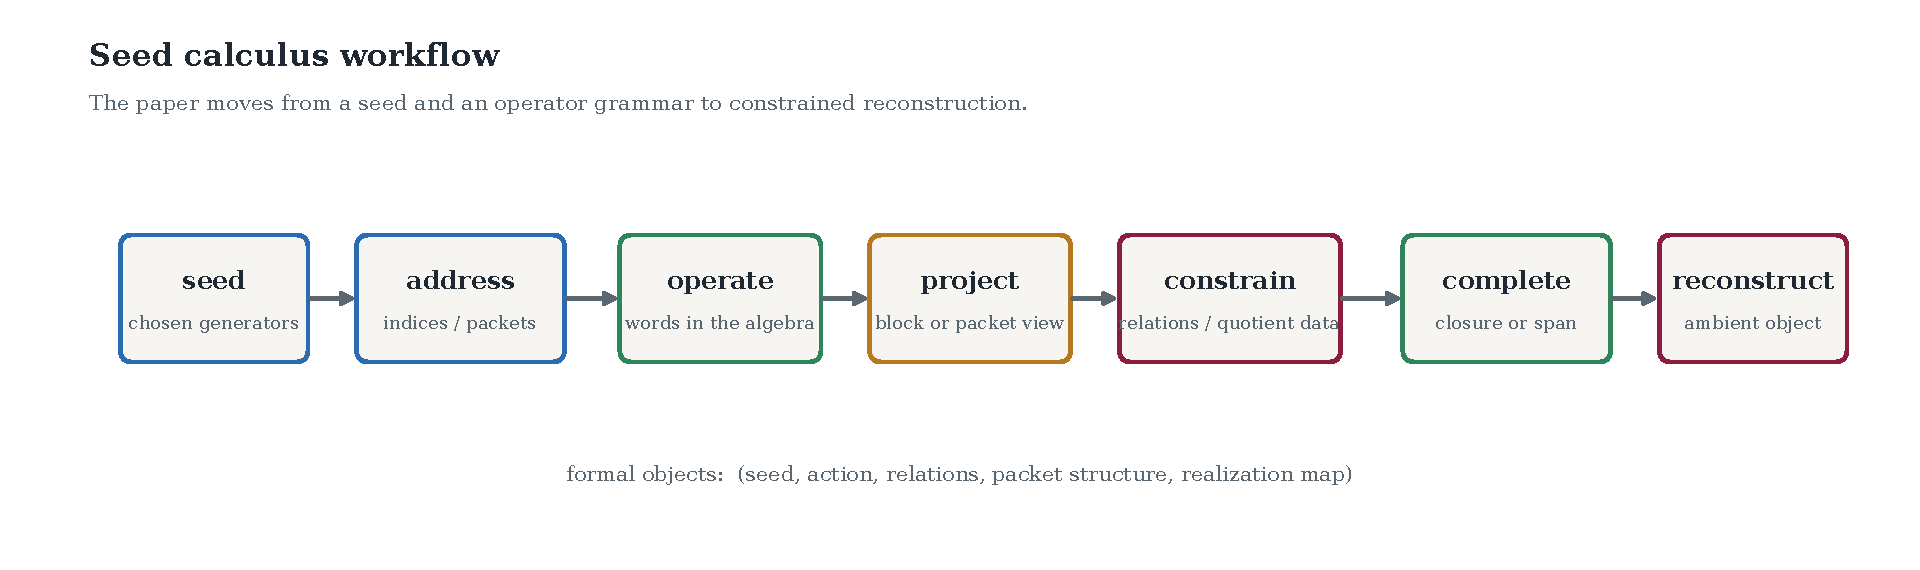
\includegraphics[width=0.96\textwidth]{01_seed_operator_grammar.pdf}
\caption{Schematic organization of the seed, operator, relation, and reconstruction data. This is a guide to the presentation, not an additional formal theorem.}
\label{fig:grammar}
\end{figure}

\subsection{What is proved here}

The paper develops the following results:
\begin{enumerate}[label=(\roman*)]
\item exact packet analysis and synthesis for finite idempotent decompositions;
\item the transfer-block decomposition and its composition law;
\item coordinate invariance under conjugation and functorial descent under intertwiners;
\item free one-seed and multi-seed presentations by operator words and relations;
\item seed-rank bounds for quotients, independent direct sums, shared direct sums, and tensor products;
\item the semisimple multiplicity formula from chosen split algebra and module equivalences;
\item the single-operator and diagonalizable multiplicity formulas from explicit block, quotient, polynomial, and eigenbasis certificates;
\item exact worked models in coordinate algebras, bounded shift systems, matrix modules, a finite typed quiver, paths, and cycles.
\end{enumerate}

\subsection{Scope and conventions}

The core is linear. Packet families are finite unless a mode of convergence
is specified, and pairwise annihilation does not mean orthogonality for an
inner product. Normed-space statements use bounded linear operators over
a nontrivially normed field; the Hilbert-space statements use $\R$ or $\C$.
Unless stated otherwise, the algebraic ground ring is a field $\bbk$.
For the semiring-valued generator inequalities, a generated hull means the
subsemimodule spanned by the seed family.

Classification results enter only through explicit data. In particular,
a chosen split algebra and module equivalence, primary generators,
polynomial projectors, scalar quotient maps, or an eigenbasis must be supplied
where the theorem requires them. Their existence is a separate classical
input. The formal development does not include a general Jordan or
Wedderburn construction, an exact eigensolver, or the projective geometry
of the coordinate-ring example. These boundaries are recorded again,
claim by claim, in the verification ledger.

\section{Typed operator grammars}

\subsection{Types, arrows, and paths}

A typed grammar is most naturally described by a directed graph. The vertices record object types, and the arrows record primitive operators that are permitted to move one type into another.

\begin{definition}[Typed linear grammar]
A typed linear grammar over a field $\bbk$ consists of a finite quiver $Q=(Q_0,Q_1)$ and, for each arrow $a:v\to w$, a declared linear operation of type $v\to w$. A realization $X$ assigns a vector space $X_v$ to each vertex and a linear map
\[
X_a:X_v\longrightarrow X_w
\]
to each arrow.
\end{definition}

Every directed path
\[
p=a_r\cdots a_1
\]
defines an address operator
\[
X_p=X_{a_r}\cdots X_{a_1}.
\]
The trivial path $e_v$ acts as the identity on $X_v$. Linear combinations of paths form the path algebra $\bbk Q$. For quiver representations, path algebras, and bound quiver algebras, see \cite{assemSimsonSkowronski2006}.

\begin{definition}[Relations]
A relation is a $\bbk$-linear combination of paths with common initial and terminal vertices. A relation ideal $I\subseteq\bbk Q$ is a two-sided ideal generated by declared relations. A realization satisfies the relations when every element of $I$ acts as zero.
\end{definition}

Thus a realization of the finite typed grammar satisfying the relations is a module over the path algebra with relations
\[
\bbk Q/I.
\]
Composition of typed operations is represented by path multiplication.

Because $Q_0$ is finite,
\[
1_{\bbk Q}=\sum_{v\in Q_0}e_v.
\]
Infinite-vertex quivers require locally unital path-algebra and module language. That extension is not used in Paper I.

\subsection{The one-space operator core}

Most theorems can be stated more transparently after collecting all types into one direct sum
\[
X=\bigoplus_{v\in Q_0}X_v.
\]
The vertex idempotent $e_v$ acts as the projector onto $X_v$, and every arrow becomes a block operator on $X$. The realized path algebra generates a unital subalgebra
\[
\cA\subseteq\End_{\bbk}(X).
\]
For topological realizations, $X$ is a Hausdorff topological vector space and $\cA$ consists of continuous operators.

\begin{definition}[Linear seed system]
A linear seed system is a tuple
\[
{
\Seed=(X,S,\cA,\cR,\cP,\tau),
}
\]
where $X$ is the ambient space, $S\subseteq X$ is a finite or controlled seed family, $\cA$ is a fixed unital operator algebra, $\cR$ is a relation system or presentation, $\cP$ is a finite packet system, and $\tau$ is a topology or completion rule.
\end{definition}

The seed family may contain one element. It is nevertheless important to allow several seeds, because the minimal required number is itself a structural invariant.

\subsection{Generated hulls}

\begin{definition}[Algebraic hull]
For $S\subseteq X$, define
\[
\Hull_{\cA}(S)
=
\Span_{\bbk}\{As:A\in\cA,\ s\in S\}.
\]
It is the smallest $\cA$-invariant subspace containing $S$. We write $\Hull_{\cA}(s)$ for $\Hull_{\cA}(\{s\})$.
\end{definition}

\begin{definition}[Topological hull]
If $X$ is topological, define
\[
\Hull_{\cA,\tau}(S)
=
\closure{\Hull_{\cA}(S)}^{\,\tau}.
\]
The seed family is topologically generating when this closure equals $X$.
\end{definition}

For a finite-dimensional Hausdorff topological vector space over $\R$ or $\C$, the algebraic hull is closed, so the algebraic and topological hulls agree. In infinite-dimensional examples, the topology is part of the theorem, not an optional afterthought.

\begin{definition}[Natural presentation]
A seed presentation is called natural relative to a declared grammar when:
\begin{enumerate}[label=(\alph*)]
\item the primitive operators are selected independently of the target element;
\item the relations are finite or effectively enumerable;
\item the topology is intrinsic to the realization;
\item no primitive operator directly stores the complete target;
\item the presentation exposes a reusable theorem, computation, or invariant.
\end{enumerate}
\end{definition}

\begin{remark}
The last condition is deliberately methodological rather than categorical. It prevents a technically valid but mathematically empty choice of a target-dependent operator $A_x$ with $A_xs=x$.
\end{remark}

\section{Free presentations by seeds and relations}

\subsection{The universal one-seed presentation}

Let $F=\bbk\langle z_1,\ldots,z_r\rangle$ be the free associative algebra. Given operators $T_1,\ldots,T_r\in\End(X)$ and a seed $s\in X$, define
\[
\Phi_s:F\longrightarrow X,
\qquad
f\longmapsto f(T_1,\ldots,T_r)s.
\]
The image is the operator hull of $s$.

\begin{theorem}[Universal one-seed presentation]
\label{thm:one-seed-presentation}
The kernel
\[
I_s=\ker\Phi_s
\]
is a left ideal of $F$, and there is a canonical isomorphism of left $F$-modules
\[
{
F/I_s\cong\Hull_F(s).
}
\]
The seed $s$ generates $X$ if and only if $\Phi_s$ is surjective. For the completion clause, let $\bbk$ be a nontrivially normed field, let $X$ be a Banach space over $\bbk$, and suppose that $F/I_s$ has been supplied with a norm for which the induced map
\[
\bar\Phi_s:F/I_s\longrightarrow X
\]
is a continuous linear isometry with dense range. Then $\bar\Phi_s$ extends uniquely to a continuous linear equivalence
\[
{\widehat{F/I_s}\simeq_L X.}
\]
If bounded operators $A$ on $F/I_s$ and $B$ on $X$ satisfy
\(
\bar\Phi_sA=B\bar\Phi_s,
\)
then the completed operator $A^\wedge$ is intertwined with $B$ by this equivalence.
\end{theorem}

\begin{proof}
For $g\in F$ and $f\in I_s$,
\[
\Phi_s(gf)=(gf)(T)s=g(T)f(T)s=0,
\]
so $I_s$ is a left ideal. The first isomorphism theorem gives
\[
F/I_s\cong\im\Phi_s=\Hull_F(s).
\]
Surjectivity is exactly the generating condition. For the final statement, a linear isometry extends uniquely from a normed space to its completion. Its extended range is dense because $\bar\Phi_s$ has dense range, and closed because the extension is an isometry into a Banach space; hence the extension is surjective and is a continuous linear equivalence. The two bounded intertwining maps agree on the dense embedded copy of $F/I_s$, so continuity makes them equal on the completion.
\end{proof}

\begin{remark}
The annihilator of a vector is generally a left ideal, not a two-sided ideal. It becomes a two-sided relation ideal in important special cases, such as a coordinate algebra generated from its multiplicative identity.
\end{remark}

\subsection{Several seeds}

\begin{theorem}[Multi-seed presentation]
\label{thm:multi-seed-presentation}
Let $S=(s_1,\ldots,s_m)$. Define
\[
\Phi_S:F^m\longrightarrow X,
\qquad
(f_1,\ldots,f_m)\longmapsto\sum_{j=1}^m f_j(T)s_j.
\]
Then $N_S=\ker\Phi_S$ is a left $F$-submodule and
\[
{
F^m/N_S\cong\Hull_F(S).
}
\]
In particular, if $X$ is finitely generated as an $F$-module, its natural-valued seed rank is the least $n\in\N$ for which there is a surjective $F$-linear map
\[
F^{(\{1,\ldots,n\})}\twoheadrightarrow X.
\]
This is the classical minimal number of module generators, commonly denoted $\mu_F(X)$; see \cite{lam1999modules}. For an arbitrary generating family indexed by $J$, the same presentation uses the direct-sum free module $F^{(J)}$.
\end{theorem}

\begin{proof}
The map $\Phi_S$ is $F$-linear. The first isomorphism theorem for modules gives the claimed quotient. A surjection from $F^n$ is determined by the images of its $n$ standard generators, and those images generate its target. Conversely, every $n$-element generating family defines such a surjection. Taking the least $n$ proves the final assertion.
\end{proof}

\subsection{Algebra generation and module generation}

Two notions must not be confused.

\begin{itemize}
\item An algebra may require several algebra generators.
\item The same algebra, regarded as a module over itself, is generated by its unit.
\end{itemize}

For example, $\bbk[x,y]$ requires the two algebra generators $x$ and $y$, but it has module seed rank one under the multiplication algebra because every polynomial is obtained by applying a multiplication operator to $1$.

This distinction will recur throughout the series. A small module seed does not imply that the operator grammar is small; both quantities must be recorded.

\section{Seed rank}

\subsection{Definition and cyclicity}

\begin{definition}[Seed rank]
The seed rank of an $\cA$-module $X$ is the least cardinal
\[
{
\srank_{\cA}(X)
=
\min\bigl\{|S|:S\subseteq X,\ \Hull_{\cA}(S)=X\bigr\}.
}
\]
For a topological module, the topological seed rank is defined analogously by
\[
\srank_{\cA,\tau}(X)
=
\min\bigl\{|S|:S\subseteq X,\ \closure{\Hull_{\cA}(S)}^{\tau}=X\bigr\}.
\]
These minima exist because $X$ itself generates under a unital action. We set
\[
\srank_{\cA}(0)=\srank_{\cA,\tau}(0)=0.
\]
For finitely generated modules the algebraic rank is a nonnegative integer; otherwise it may be an infinite cardinal. Algebraically, this is the standard invariant $\mu_{\cA}(X)$, with the term \emph{seed rank} retaining the declared operator algebra as part of the datum \cite{lam1999modules}.
A vector $s$ is cyclic when $\Hull_{\cA}(s)=X$.
\end{definition}

\begin{proposition}[Cyclic characterization]
\label{prop:cyclic-characterization}
For a nonzero module $X$,
\[
\srank_{\cA}(X)=1
\quad\Longleftrightarrow\quad
X\text{ contains a cyclic vector.}
\]
\end{proposition}

\begin{proof}
A cyclic vector gives a one-element generating set. Conversely, a generating set of cardinality one consists of a cyclic vector. Since $X$ is nonzero, the empty family does not generate.
\end{proof}

\subsection{Functorial bounds}

\begin{theorem}[Quotient monotonicity]
\label{thm:quotient}
Let $\varphi:\cA\to\cB$ be an algebra homomorphism and let $\Phi:X\twoheadrightarrow Y$ be a surjective $\varphi$-semilinear map, so that
\[
\Phi(Ax)=\varphi(A)\Phi(x)
\]
for all $A\in\cA$ and $x\in X$. Then
\[
{
\srank_{\cB}(Y)\le \srank_{\cA}(X).
}
\]
\end{theorem}

\begin{proof}
If $S$ generates $X$, then every $y\in Y$ has the form $y=\Phi(x)$ with
\[
x=\sum_j A_js_j.
\]
Therefore
\[
y=\sum_j\varphi(A_j)\Phi(s_j),
\]
so $\Phi(S)$ generates $Y$.
\end{proof}

\begin{corollary}[Isomorphism invariance over the image algebra]
\label{cor:image-algebra-invariance}
If $\Phi:X\to Y$ is a linear isomorphism satisfying the hypotheses of \cref{thm:quotient}, then
\[
\srank_{\varphi(\cA)}(Y)=\srank_{\cA}(X).
\]
In particular, seed rank relative to $\cB$ is preserved when $\varphi:\cA\to\cB$ is an algebra isomorphism.
\end{corollary}

\begin{proof}
For every $S\subseteq X$, the intertwining identity gives
\[
\Phi\bigl(\Hull_{\cA}(S)\bigr)
=
\Hull_{\varphi(\cA)}(\Phi S).
\]
Because $\Phi$ bijects generating families and preserves their cardinalities, taking the two minima gives the equality. Equality relative to the full target algebra $\cB$ requires $\varphi(\cA)=\cB$.
\end{proof}

\begin{proposition}[Shared direct-sum bound]
\label{prop:shared-direct-sum}
If one algebra $\cA$ acts diagonally on $X\oplus Y$, then
\[
{
\srank_{\cA}(X\oplus Y)
\le
\srank_{\cA}(X)+\srank_{\cA}(Y).
}
\]
\end{proposition}

\begin{proof}
Embed a generating family for $X$ as vectors $(x_i,0)$ and a generating family for $Y$ as vectors $(0,y_j)$. Their union generates the direct sum.
\end{proof}

\begin{theorem}[Independent direct-sum formula]
\label{thm:independent-direct-sum}
Let $\cA$ act on $X$ and $\cB$ act on $Y$. Under the product algebra $\cA\times\cB$,
\[
{
\srank_{\cA\times\cB}(X\oplus Y)
=
\max\{\srank_{\cA}(X),\srank_{\cB}(Y)\}.
}
\]
\end{theorem}

\begin{proof}
Projection onto either summand is an intertwining quotient, so the seed rank of the direct sum is at least the maximum. Conversely, let $r$ be the maximum cardinal. Choose generating families realizing the two minima, embed their index sets into a common index set $K$ of cardinality $r$, and pad the missing positions with zero. If $(x_k)_{k\in K}$ generates $X$ and $(y_k)_{k\in K}$ generates $Y$, then the $r$ vectors $(x_k,y_k)$ generate $X\oplus Y$, because elements of $\cA\times\cB$ act independently on the two coordinates.
\end{proof}

\begin{proposition}[Tensor-product bound]
\label{prop:tensor-product-bound}
Let $\bbk$ be a commutative semiring, let $\cA$ and $\cB$ be $\bbk$-algebras, and let $X$ and $Y$ carry compatible $\bbk$-module and respectively $\cA$-module and $\cB$-module structures, including the usual scalar-tower and commuting-action laws. All tensor products below are over $\bbk$. Under the natural action determined by
\[
(a\otimes b)(x\otimes y)=(ax)\otimes(by),
\]
\[
{
\srank_{\cA\otimes\cB}(X\otimes Y)
\le
\srank_{\cA}(X)\srank_{\cB}(Y).
}
\]
\end{proposition}

\begin{proof}
Choose generating families $(x_i)_{i\in I}$ for $X$ and $(y_j)_{j\in J}$ for $Y$. For arbitrary $x\in X$ and $y\in Y$, there are finite subsets $I_0\subseteq I$ and $J_0\subseteq J$ and operators $A_i\in\cA$, $B_j\in\cB$ such that
\[
x=\sum_{i\in I_0}A_ix_i,
\qquad
y=\sum_{j\in J_0}B_jy_j.
\]
Therefore
\[
x\otimes y
=
\sum_{i\in I_0}\sum_{j\in J_0}
(A_i\otimes B_j)(x_i\otimes y_j).
\]
Since simple tensors span $X\otimes Y$, the family $\{x_i\otimes y_j:(i,j)\in I\times J\}$ generates. Minimizing over the two generating families gives the stated cardinal bound.
\end{proof}

\begin{boundary}
The tensor bound need not be an equality. Its value depends on the acting algebra and on relations among the tensor factors; no refinement hypothesis enters the foundational inequality.
\end{boundary}

\subsection{Quotient witnesses and lower bounds}

Quotients provide a systematic way to prove that a proposed seed family is too small.

\begin{definition}[Seed-rank witness]
An intertwining quotient $\Phi:X\twoheadrightarrow Y$ is a seed-rank witness of order $r$ when $\srank(Y)=r$. By quotient monotonicity it certifies
\[
\srank(X)\ge r.
\]
\end{definition}

\begin{proposition}[Scalar quotient obstruction]
\label{prop:scalar-quotient-obstruction}
Let $\chi:\cA\to_{\bbk}\bbk$ be a character, let $Y$ be a finite-dimensional $\bbk$-space, and suppose there is a surjective $\chi$-semilinear map $\Phi:X\twoheadrightarrow Y$. Equivalently,
\[
\Phi(Ax)=\chi(A)\Phi(x).
\]
If $r=\dim_{\bbk}Y$, then
\[
{\srank_{\cA}(X)\ge r.}
\]
\end{proposition}

\begin{proof}
The orbit of a vector in $Y$ is contained in its span, which has dimension at most one, because all operators act scalarly. Therefore $r$ independent quotient directions require at least $r$ image seeds. Apply quotient monotonicity.
\end{proof}

\begin{example}[Primary quotient]
In the classical finite-dimensional primary decomposition, the quotient
\[
X_{\lambda}/(T-\lambda I)X_{\lambda}
\]
is a scalar $\bbk[T]$-module. A chosen identification of this quotient with
$\bbk^{m_{\lambda}}$ supplies the surjective scalar-quotient map used in
\cref{thm:single-operator}. For Jordan data, classical canonical-form theory
identifies $m_{\lambda}$ with both the number of blocks at $\lambda$ and
$\dim\ker(T-\lambda I)$. That identification is an input when the formal
certificate is instantiated, rather than a conclusion of the kernel-checked
declaration.
\end{example}

\begin{remark}
This formulation is useful beyond Jordan theory. To prove a lower bound, one does not need to understand the entire generated object. It is enough to identify a quotient in which the operator grammar loses its ability to mix independent directions.
\end{remark}

\section{The semisimple multiplicity theorem}

The first substantial closed formula for seed rank appears once a split-product decomposition has been fixed. The classical Wedderburn--Artin theorem and the standard description of modules over full matrix algebras provide such data in the usual finite-dimensional split-semisimple setting \cite{lam2001noncommutative}\cite{lam1999modules}. The theorem below makes the data explicit: it proves the formula after an algebra equivalence and a compatible module equivalence have been supplied; it does not assert the classification theorem that produces them.

\begin{theorem}[Semisimple multiplicity formula]
\label{thm:semisimple}
Let $I$ be a nonempty finite index set, let $\bbk$ be a field, and let $\cA$ be a unital $\bbk$-algebra acting on $X$. Suppose there is a chosen $\bbk$-algebra equivalence
\[
\theta:\cA\simeq_{\bbk}\prod_{i\in I}M_{d_i}(\bbk)
\]
and a chosen $\theta$-semilinear equivalence
\[
E:X\simeq_{\theta}\prod_{i\in I}M_{d_i\times m_i}(\bbk).
\]
Assume $d_i\ge1$ for every $i$. Then
\[
{
\srank_{\cA}(X)
=
\max_{i\in I}
\left\lceil\frac{m_i}{d_i}\right\rceil.
}
\]
\end{theorem}

\begin{proof}
Transport along $\theta$ and $E$, so it is enough to work in the displayed literal product. A vector in its $i$th component is a $d_i\times m_i$ matrix $V$. The orbit $M_{d_i}(\bbk)V$ consists of matrices whose row space lies in the row space of $V$. Consequently one seed can expose at most $d_i$ independent directions in the multiplicity space $\bbk^{m_i}$.

If $r$ vectors generate $X_i$, the union of their row spaces must span $\bbk^{m_i}$. Its dimension is at most $rd_i$, so
\[
r\ge\left\lceil\frac{m_i}{d_i}\right\rceil.
\]
This gives the lower bound after taking the maximum over $i$.

For the converse, let
\[
r=\max_i\left\lceil\frac{m_i}{d_i}\right\rceil.
\]
For each $i$, choose $r$ matrices whose combined row spaces span $\bbk^{m_i}$; this is possible because $rd_i\ge m_i$. Combine the $j$th chosen matrix from every component into one vector of the product. The product algebra acts independently on the components, so these $r$ vectors generate the product module. Seed rank is invariant under the supplied compatible semilinear equivalence, which transports the equality back to $X$.
\end{proof}

\begin{boundary}[Classification input]
Over an algebraically closed field, finite-dimensional split semisimple algebras and their finite-dimensional modules admit equivalences of the displayed form by classical structure theory. That existence statement is cited background. The kernel-checked theorem begins with the particular equivalences $\theta$ and $E$ as input.
\end{boundary}

\begin{corollary}[Full matrix algebra]
\label{cor:full-matrix}
For any field $\bbk$ and $n\ge1$, the natural module $\bbk^n$ over $M_n(\bbk)$ satisfies
\[
\srank_{M_n(\bbk)}(\bbk^n)=1.
\]
More strongly, every nonzero vector is cyclic.
\end{corollary}

\begin{proof}
If $v\ne0$ and $w\in\bbk^n$, choose a linear functional $\phi$ with $\phi(v)=1$. The rank-one operator $w\phi$ sends $v$ to $w$, so $v$ is cyclic. Since the module is nonzero, its seed rank is one.
\end{proof}

\begin{corollary}[Multiplicity obstruction]
\label{cor:multiplicity-obstruction}
For $d\ge1$ and $m\ge0$, the diagonal action of $M_d(\bbk)$ on $(\bbk^d)^{\oplus m}$ satisfies
\[
\srank=\left\lceil\frac md\right\rceil.
\]
Thus repeated copies of one irreducible packet create a genuine lower bound even though each individual copy is cyclic.
\end{corollary}

\begin{figure}[htbp]
\centering
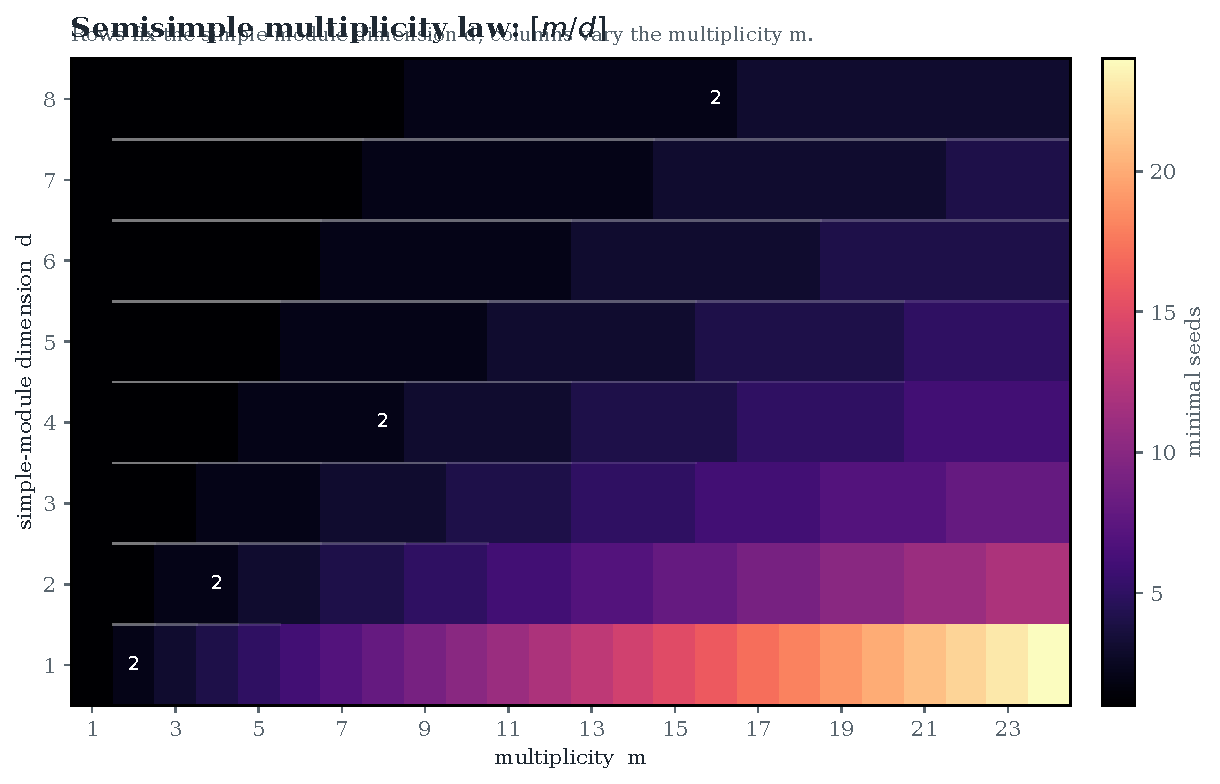
\includegraphics[width=0.84\textwidth]{04_semisimple_seed_rank.pdf}
\caption{The semisimple multiplicity formula for one simple block. A seed can expose at most $d$ independent multiplicity directions, so $m$ copies require $\lceil m/d\rceil$ seeds.}
\label{fig:semisimple}
\end{figure}

\begin{remark}[Non-algebraically-closed fields]
The stated theorem works over any field once the displayed split matrix-algebra and module equivalences are supplied. A general semisimple algebra over a non-splitting field can instead involve nontrivial division algebras of endomorphisms, and its intrinsic formula must use dimensions over those division algebras; see \cite{lam2001noncommutative}.
\end{remark}

\section{One operator and the cyclic-vector theorem}

A single linear operator $T$ generates the commutative algebra $\bbk[T]$.
The generator argument can be separated cleanly from the classification
theorem that produces primary or Jordan data.  We therefore state the
kernel-checked result from an explicit certificate.  Classical
$\bbk[t]$-module, primary-decomposition, and canonical-form theory explains
how such certificates arise in the standard finite-dimensional setting
\cite{roman2008}; see also \cite{hornJohnson2012}.

\begin{theorem}[Single-operator seed number from primary data]
\label{thm:single-operator}
Let $\bbk$ be a field, let $T\in\End_{\bbk}(X)$, and let $\Lambda$ be a
nonempty finite label set.  Suppose the following data are supplied:
\begin{enumerate}[label=(\roman*)]
\item numbers $m_{\lambda}\in\N$, scalars $a_{\lambda}\in\bbk$, and vectors
$v_{\lambda,j}\in X$ for $1\le j\le m_{\lambda}$ such that
\[
X=\Span_{\bbk}\{p(T)v_{\lambda,j}:
  \lambda\in\Lambda,\ 1\le j\le m_{\lambda},\ p\in\bbk[t]\};
\]
\item a number $R\in\N$ with $m_{\lambda}\le R$ for all $\lambda$ and
$m_{\lambda_*}=R$ for some $\lambda_*\in\Lambda$;
\item padded vectors
\[
w_j=\sum_{\lambda:\,j\le m_{\lambda}}v_{\lambda,j},
\qquad 1\le j\le R,
\]
and, for every admissible $(\lambda,j)$, a polynomial
$e_{\lambda,j}\in\bbk[t]$ satisfying
\[
e_{\lambda,j}(T)w_j=v_{\lambda,j};
\]
\item surjective linear maps
$q_{\lambda}:X\twoheadrightarrow\bbk^{m_{\lambda}}$ satisfying
\[
q_{\lambda}\bigl(p(T)x\bigr)
=p(a_{\lambda})q_{\lambda}(x)
\qquad(p\in\bbk[t],\ x\in X).
\]
\end{enumerate}
Then $R$ is the least natural number $r$ for which $r$ polynomial-orbit
seeds generate $X$:
\[
{
R=\min\left\{r\in\N:
\begin{array}{l}
\text{there exist }u_1,\ldots,u_r\in X\text{ with}\\[2pt]
X=\Span_{\bbk}\{p(T)u_j:p\in\bbk[t],\ 1\le j\le r\}
\end{array}
\right\}.
}
\]
Moreover, for the genuine image algebra
\[
\bbk[T]=\operatorname{alg}_{\bbk}\langle T\rangle
\subseteq\End_{\bbk}(X),
\]
polynomial-orbit generation is exactly module generation, and therefore
\[
{
\mu_{\bbk[T]}(X)=R,
\qquad
\srank_{\bbk[T]}(X)=(R:\operatorname{Cardinal}).
}
\]
\end{theorem}

\begin{proof}
The extraction polynomials recover every $v_{\lambda,j}$ from the padded
family $(w_j)_{j=1}^{R}$.  The joint-generation hypothesis therefore shows
that these $R$ vectors generate $X$.  Conversely, suppose $r$ vectors
generate.  Their images under $q_{\lambda}$ generate
$\bbk^{m_{\lambda}}$, but the displayed intertwining identity makes every
polynomial act there by a scalar.  Hence $m_{\lambda}\le r$ for every
$\lambda$.  Applying this at $\lambda_*$ gives $R\le r$.  Finally,
the algebra generated by $T$ is the range of polynomial evaluation
$p\mapsto p(T)$.  Hence the $\bbk[T]$-span of any seed family, after
restriction to $\bbk$, equals its polynomial-orbit span.  This identifies the
least natural number with the canonical module seed finrank and cardinal seed
rank.
\end{proof}

\begin{corollary}[Certified cyclic matrix criterion]
\label{cor:cyclic-matrix-criterion}
Assume the hypotheses of \cref{thm:single-operator}, that $X$ is
finite-dimensional, and that $m_{\lambda}>0$ for every $\lambda$.  Supply
block counts $b_{\lambda}\in\N$ together with the two canonical-form bridges
\[
m_{\lambda}=b_{\lambda}\quad(\lambda\in\Lambda),
\qquad
m_T(t)=\chi_T(t)
\quad\Longleftrightarrow\quad
b_{\lambda}=1\text{ for every }\lambda,
\]
where $m_T$ and $\chi_T$ are the minimal and characteristic polynomials.
Then the following four conditions are equivalent:
\begin{enumerate}[label=(\roman*)]
\item $T$ has a cyclic vector;
\item $m_{\lambda}=1$ for every $\lambda$;
\item $b_{\lambda}=1$ for every $\lambda$;
\item $m_T=\chi_T$.
\end{enumerate}
\end{corollary}

\begin{proof}
By \cref{thm:single-operator}, cyclicity is equivalent to $R=1$.  Positivity,
the bounds $m_{\lambda}\le R$, and the equality
$m_{\lambda_*}=R$ make this equivalent to
$m_{\lambda}=1$ for every $\lambda$.  The first supplied bridge identifies
this with one block per label, and the second identifies that condition with
$m_T=\chi_T$.
\end{proof}

\begin{boundary}[Canonical-form input]
For a finite-dimensional operator over an algebraically closed field,
classical primary and Jordan theory supplies the preceding certificate with
$m_{\lambda}=\dim\ker(T-\lambda I)$ and supplies the polynomial bridge.
Consequently the usual geometric-multiplicity formula and four-way
nonderogatory criterion follow classically.  The Lean declarations verify
the generator inequalities, extraction argument, and certified cyclicity
criterion; they do not construct the Jordan decomposition or prove those
identifications from the bare hypotheses on $T$.
\end{boundary}

\begin{example}[Companion operator]
For a companion matrix of size $n\ge1$, use the convention in which
$e_1$ is the first coordinate vector and
\[
e_1,Te_1,\ldots,T^{n-1}e_1
\]
is a basis. This Krylov basis proves cyclicity over the ground field,
without a splitting hypothesis. It does not by itself supply the scalar
primary data of \cref{thm:single-operator}. The nilpotent companion used in
the computational example has one primary block at zero, so it also
admits that theorem's certificate with $R=1$.
\end{example}

\begin{example}[Repeated primary blocks]
Let $m\ge1$ and
\[
T=J_m(\lambda)\oplus J_m(\lambda).
\]
Then
\[
\dim\ker(T-\lambda I)=2,
\]
and the standard primary certificate has $m_{\lambda}=2$.  Its scalar
quotient forces at least two seeds, while the two block generators supply the
matching upper bound.  A single vector with nonzero components in both blocks
produces only a linked combination of their two chains and cannot separate
them.
\end{example}

\begin{figure}[htbp]
\centering
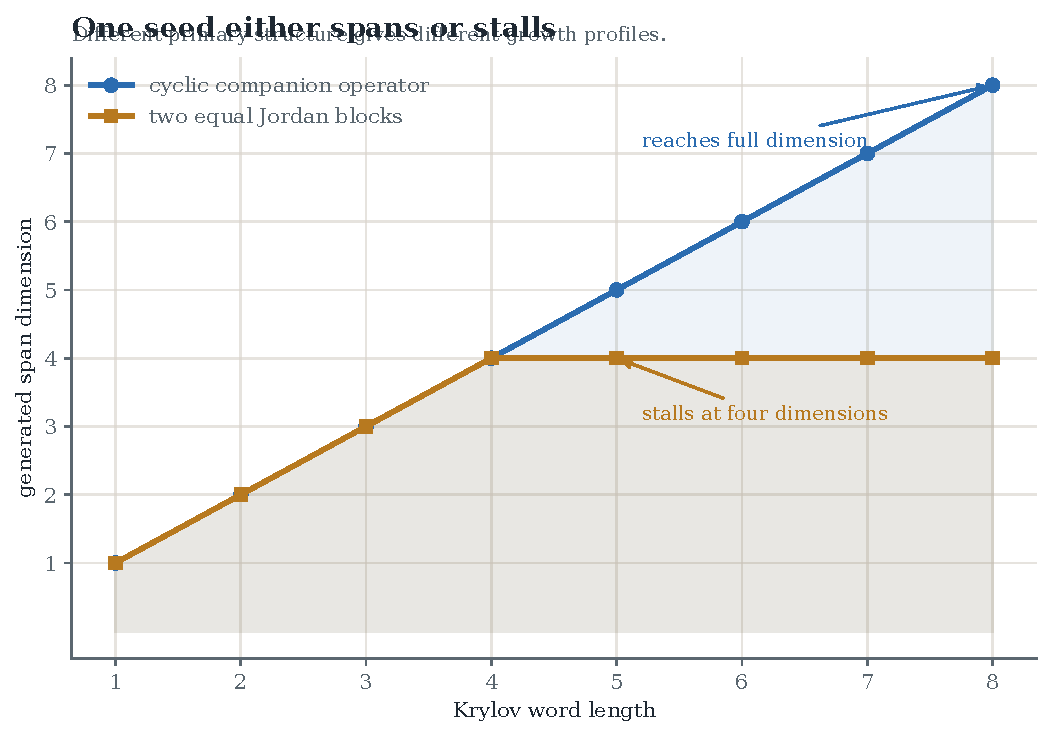
\includegraphics[width=0.79\textwidth]{03_cyclic_rank_profiles.pdf}
\caption{Krylov rank profiles for a cyclic companion operator and for two equal primary blocks. The second orbit stalls before reaching the ambient dimension because one seed cannot separate the repeated blocks.}
\label{fig:krylov}
\end{figure}

\section{Exact packet systems}

\subsection{Idempotent coordinates}

\begin{definition}[Finite packet system]
A finite packet system on $X$ is a family indexed by a finite set $I$,
\[
\cP=\{P_{\alpha}\}_{\alpha\in I}
\subseteq\End(X)
\]
satisfying
\[
P_{\alpha}P_{\beta}=\delta_{\alpha\beta}P_{\alpha},
\qquad
\sum_{\alpha\in I}P_{\alpha}=I.
\]
The packet space is $X_{\alpha}=P_{\alpha}X$.
\end{definition}

Orthogonality with respect to an inner product is useful but not required. Pairwise annihilation and completeness already imply the algebraic direct sum
\[
X=\bigoplus_{\alpha\in I}X_{\alpha}.
\]

\begin{definition}[Analysis and synthesis]
Define
\[
\mathcal A_{\cP}:X\longrightarrow\bigoplus_{\alpha}X_{\alpha},
\qquad
\mathcal A_{\cP}x=(P_{\alpha}x)_{\alpha},
\]
and
\[
\mathcal S_{\cP}:\bigoplus_{\alpha}X_{\alpha}\longrightarrow X,
\qquad
\mathcal S_{\cP}(x_{\alpha})_{\alpha}=\sum_{\alpha}x_{\alpha}.
\]
\end{definition}

\begin{theorem}[Exact packet coordinates]
\label{thm:analysis-synthesis}
For every finite packet system,
\[
{
\mathcal S_{\cP}\mathcal A_{\cP}=I_X,
\qquad
\mathcal A_{\cP}\mathcal S_{\cP}=I_{\oplus X_{\alpha}}.
}
\]
Hence analysis and synthesis are inverse coordinate maps.
\end{theorem}

\begin{proof}
Completeness gives
\[
\mathcal S_{\cP}\mathcal A_{\cP}x
=
\sum_{\alpha}P_{\alpha}x=x.
\]
If $x_{\alpha}\in X_{\alpha}$, then
\[
P_{\beta}\sum_{\alpha}x_{\alpha}
=
\sum_{\alpha}P_{\beta}P_{\alpha}x_{\alpha}
=x_{\beta}.
\]
Therefore the analysis of the synthesis returns the original packet tuple.
\end{proof}

\begin{corollary}[Packetwise equality]
\label{cor:packetwise-equality}
Two vectors $x,y\in X$ are equal if and only if
\[
P_{\alpha}x=P_{\alpha}y
\]
for every packet $\alpha$.
\end{corollary}

\begin{boundary}[Infinite packet systems]
For infinitely many packets, the equation
\[
\sum_{\alpha}P_{\alpha}=I
\]
requires a declared mode of convergence. Strong, weak, unconditional, formal, and $p$-adic convergence are different statements. Paper I uses finite packets or explicitly convergent examples.
\end{boundary}

\subsection{Continuous packets and closed ranges}

The finite packet theorem extends cleanly to Banach and Hilbert spaces when the projectors are bounded. We use standard conventions for continuous linear maps, closed subspaces, and completion \cite{schaeferWolff1999}\cite{conway1990}.

\begin{theorem}[Topological packet isomorphism]
\label{thm:topological-packets}
Let $X$ be a Banach space and let $(P_i)_{i\in I}$ be a finite family of bounded pairwise annihilating idempotents with sum $I$. Then each packet $X_i=P_iX$ is closed, and analysis is a continuous linear equivalence
\[
{
\mathcal A_{\cP}:X\simeq_L\prod_{i\in I}X_i
}
\]
for the standard finite dependent-product norm, with inverse the finite-sum synthesis map $\mathcal S_{\cP}$.
\end{theorem}

\begin{proof}
Since
\[
X_i=\im P_i=\ker(I-P_i),
\]
and $I-P_i$ is continuous, $X_i$ is closed. Each coordinate of analysis is bounded, and synthesis is a finite sum of bounded coordinate inclusions. The algebraic inverse identities from \cref{thm:analysis-synthesis} therefore package these maps as the displayed continuous linear equivalence.
\end{proof}

\begin{corollary}[Completion preserves a finite packet split]
\label{cor:completion-packet-split}
Let $X$ be a normed space, let $M\subseteq X$ be a dense linear subspace, and let $P_i$ be a bounded idempotent. Then
\[
{\closure{P_iM}=P_iX.}
\]
For a finite bounded packet family this holds for every packet, so packet extraction commutes with completion in this precise sense. No invariance hypothesis $P_iM\subseteq M$ is needed for the equality.
\end{corollary}

\begin{proof}
Because $P_iX=\ker(I-P_i)$ is closed and contains $P_iM$, one has $\closure{P_iM}\subseteq P_iX$. Conversely, approximate any $x\in X$ by elements of $M$ and use continuity of $P_i$ to obtain $P_ix\in\closure{P_iM}$.
\end{proof}

\begin{remark}
This corollary is the precise reason the bilateral-shift example may be proved on finite-support sequences and then completed in $\ell^2$. It also records a limitation: if the projectors are unbounded or the packet sum is infinite and conditional, completion need not commute with packet extraction.
\end{remark}

\subsection{Transfer blocks}

The following formulas are ordinary block-matrix identities relative to $X=\bigoplus_{\alpha}X_{\alpha}$, written in packet notation; compare \cite{hornJohnson2012}.

\begin{definition}[Transfer block]
For $T\in\End(X)$ define
\[
{
T_{\beta\alpha}=P_{\beta}TP_{\alpha}.
}
\]
It maps the input packet $X_{\alpha}$ into the output packet $X_{\beta}$.
\end{definition}

\begin{theorem}[Exact operator reconstruction]
\label{thm:operator-reconstruction}
Every operator has the exact decomposition
\[
{
T=\sum_{\alpha,\beta}T_{\beta\alpha}.
}
\]
\end{theorem}

\begin{proof}
Insert the identity on both sides of $T$:
\[
T
=
\left(\sum_{\beta}P_{\beta}\right)
T
\left(\sum_{\alpha}P_{\alpha}\right)
=
\sum_{\alpha,\beta}P_{\beta}TP_{\alpha}.
\]
\end{proof}

\begin{theorem}[Packet matrix multiplication]
\label{thm:block-composition}
If $S,T\in\End(X)$, then
\[
{
(ST)_{\gamma\alpha}
=
\sum_{\beta}S_{\gamma\beta}T_{\beta\alpha}.
}
\]
Thus packet blocks compose by ordinary matrix multiplication over operator-valued entries.
\end{theorem}

\begin{proof}
Insert completeness between the two operators:
\[
P_{\gamma}STP_{\alpha}
=
P_{\gamma}S
\left(\sum_{\beta}P_{\beta}\right)
TP_{\alpha}
=
\sum_{\beta}
(P_{\gamma}SP_{\beta})(P_{\beta}TP_{\alpha}).
\]
\end{proof}

\begin{corollary}[Packet powers]
\label{cor:packet-powers}
For $m\ge1$,
\[
(T^m)_{\beta\alpha}
=
\sum_{\alpha=\alpha_0,\ldots,\alpha_m=\beta}
T_{\alpha_m\alpha_{m-1}}
\cdots
T_{\alpha_1\alpha_0}.
\]
The sum is over all packet paths of length $m$ from $\alpha$ to $\beta$.
\end{corollary}

\begin{proof}
Iterate \cref{thm:block-composition}.
\end{proof}

\begin{corollary}[Adjoint reversal]
\label{cor:adjoint-reversal}
If $X$ is a Hilbert space, the projectors are orthogonal, and $T:X\to X$ is bounded, then
\[
(T_{\beta\alpha})^*=(T^*)_{\alpha\beta}.
\]
\end{corollary}

\begin{proof}
Use $P_{\alpha}^*=P_{\alpha}$:
\[
(P_{\beta}TP_{\alpha})^*=P_{\alpha}T^*P_{\beta}.
\]
\end{proof}

\begin{theorem}[Algebraic full block representation]
\label{thm:block-algebra}
Restriction of the transfer blocks gives an algebra isomorphism
\[
{
\End_{\bbk}(X)
\cong
\prod_{\beta,\alpha}\Hom_{\bbk}(X_{\alpha},X_{\beta}),
}
\]
where the dependent family on the right carries the transported algebra structure, and its multiplication is exactly the output-first block law
\[
(BC)_{\gamma\alpha}=\sum_{\beta}B_{\gamma\beta}C_{\beta\alpha}.
\]
\end{theorem}

\begin{proof}
The map from an operator to its block restrictions is injective by exact reconstruction. Given an arbitrary family of maps $B_{\beta\alpha}:X_{\alpha}\to X_{\beta}$, define
\[
T\left(\sum_{\alpha}x_{\alpha}\right)
=
\sum_{\alpha,\beta}B_{\beta\alpha}x_{\alpha}.
\]
The sum is finite and therefore defines an operator with the prescribed blocks. Compatibility with multiplication is \cref{thm:block-composition}.
\end{proof}

\begin{remark}[Bounded block representation]
If $X$ is Banach and the finite packet projectors are bounded, bounded operators correspond to finite matrices of bounded packet maps. Arbitrary algebraic block maps need not define bounded operators.
\end{remark}

\begin{corollary}[Dimension count]
\label{cor:block-dimension-count}
If $X$ is finite-dimensional and $d_{\alpha}=\dim X_{\alpha}$, then
\[
\dim\End(X)
=
\sum_{\alpha,\beta}d_{\alpha}d_{\beta}
=
\left(\sum_{\alpha}d_{\alpha}\right)^2.
\]
\end{corollary}

\begin{definition}[Support relation]
For a relation $R\subseteq I\times I$, let
\[
\mathcal M_R
=
\{T\in\End(X):T_{\beta\alpha}=0
\text{ whenever }(\alpha,\beta)\notin R\}.
\]
\end{definition}

\begin{theorem}[When an algebraic packet support pattern is an algebra]
\label{thm:block-support-algebra}
Assume every packet space is nonzero. The space $\mathcal M_R$ contains the identity precisely when $R$ is reflexive. It is closed under multiplication for all allowed block maps precisely when $R$ is transitive. Hence reflexive transitive relations, or packet preorders, are exactly the universal zero patterns defining unital block-support algebras.
\end{theorem}

\begin{proof}
The identity has nonzero diagonal block $I_{X_{\alpha}}$, so all pairs $(\alpha,\alpha)$ must belong to $R$. If $R$ is transitive and $S,T$ are supported on $R$, then a nonzero term
\[
S_{\gamma\beta}T_{\beta\alpha}
\]
can occur only when $(\alpha,\beta)$ and $(\beta,\gamma)$ belong to $R$, hence $(\alpha,\gamma)\in R$. The block-composition formula gives closure.

Conversely, if transitivity fails, choose $(\alpha,\beta),(\beta,\gamma)\in R$ with $(\alpha,\gamma)\notin R$. Since the packet spaces are nonzero, choose rank-one maps $T:X_{\alpha}\to X_{\beta}$ and $S:X_{\beta}\to X_{\gamma}$ with $ST\ne0$. Then $S,T\in\mathcal M_R$ but $ST\notin\mathcal M_R$.
\end{proof}

\begin{remark}
The converse is algebraic. In a category of bounded or continuous operators, it additionally requires enough continuous rank-one maps to detect a failed composite edge.
\end{remark}

\begin{figure}[htbp]
\centering
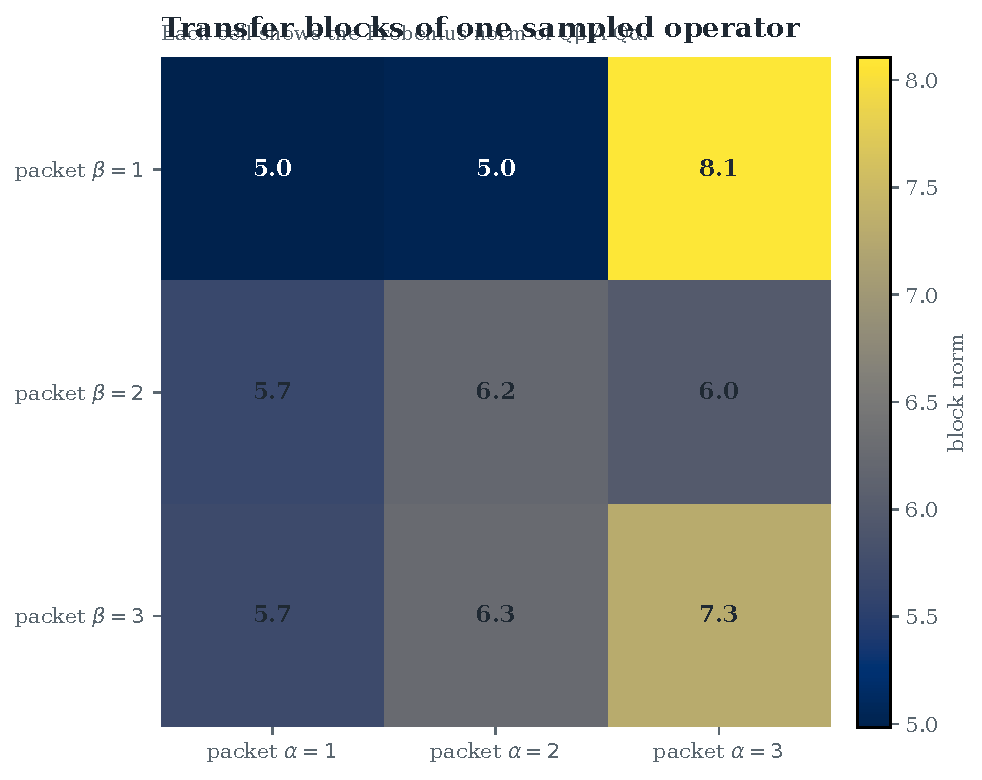
\includegraphics[width=0.72\textwidth]{02_transfer_block_norms.pdf}
\caption{An operator represented by its packet-to-packet block norms. The diagonal entries preserve packets; off-diagonal entries transfer information between packets.}
\label{fig:transfer-blocks}
\end{figure}

\subsection{Transfer graphs and reachability}

\begin{definition}[Transfer graph]
For a generating operator family $\cO$, the transfer graph has packet vertices $I$ and an edge
\[
\alpha\longrightarrow\beta
\]
when
\[
P_{\beta}OP_{\alpha}\ne0
\]
for at least one $O\in\cO$.
\end{definition}

\begin{proposition}[Reachability obstruction]
\label{prop:reachability-obstruction}
Let $H$ be the algebraic word-orbit hull of a seed family supported in packets belonging to $S_0\subseteq I$. Then $H$ lies in the submodule supported on the reflexive-transitive set of vertices reachable from $S_0$. In particular, if a nonzero packet is not reachable, then $H\ne X$.

For the topological extension, let the realization be normed and let $Q$ be a nonzero bounded packet projector. Once the algebraic argument has established $H\subseteq\ker Q$, continuity gives
\[
{\closure H\subseteq\ker Q,\qquad \closure H\ne X.}
\]
\end{proposition}

\begin{proof}
Induction on an operator word shows that reachable support is invariant under every grammar operator. Spanning the word orbit therefore gives the algebraic inclusion. A nonzero unreachable projector annihilates that support, so the hull is proper. In the topological clause, $\ker Q$ is closed because $Q$ is bounded. It contains $H$, hence also $\closure H$; if $\closure H=X$, then $Q$ would vanish identically, contradicting $Q\ne0$.
\end{proof}

\begin{remark}
A seed may have components in several packets. A count of source strongly connected components therefore gives a lower bound only when each seed is supported in a single packet and every counted component contains a nonzero packet. Reachability alone does not determine the minimum size of an unrestricted seed family.
\end{remark}

\section{Coordinate transport and naturality}

\subsection{Conjugate packet systems}

Let $U:X\to Y$ be an isomorphism. Transport the packet system and an operator by
\[
Q_{\alpha}=UP_{\alpha}U^{-1},
\qquad
T^U=UTU^{-1}.
\]

\begin{theorem}[Coordinate transport]
\label{thm:coordinate-transport}
The family $\{Q_{\alpha}\}$ is a packet system on $Y$, and its transfer blocks satisfy
\[
{
Q_{\beta}T^UQ_{\alpha}
=
U(P_{\beta}TP_{\alpha})U^{-1}.
}
\]
Thus packet identities, every zero/nonzero transfer edge, and reflexive-transitive reachability are invariant under coordinate transport.
\end{theorem}

\begin{proof}
Conjugation preserves products and sums:
\[
Q_{\alpha}Q_{\beta}
=
UP_{\alpha}P_{\beta}U^{-1}
=
\delta_{\alpha\beta}Q_{\alpha},
\]
while
\[
\sum_{\alpha}Q_{\alpha}=UIU^{-1}=I.
\]
The block formula follows by direct multiplication.
\end{proof}

\begin{figure}[htbp]
\centering
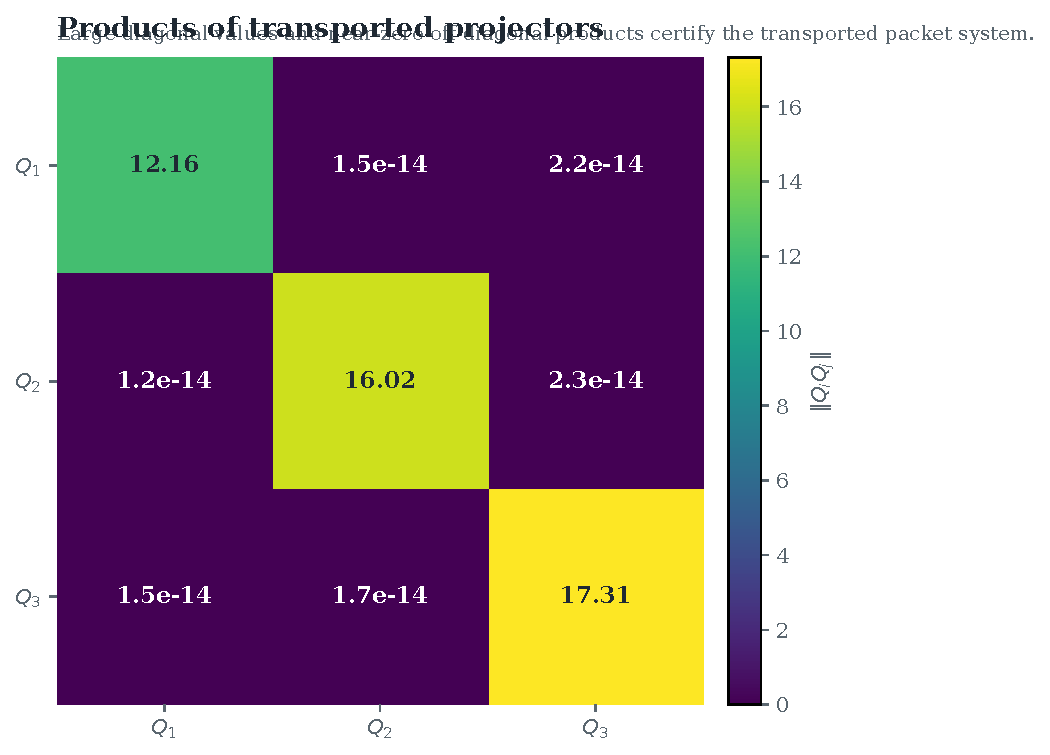
\includegraphics[width=0.72\textwidth]{09_coordinate_transport.pdf}
\caption{Numerical certificate for a nonorthogonal transported packet system. The diagonal products retain idempotent size while off-diagonal products remain at roundoff level.}
\label{fig:coordinate-transport}
\end{figure}

\subsection{Intertwining morphisms}

\begin{definition}[Strict morphism of seed systems]
Let $(X,\cA,(P_{\alpha})_{\alpha\in I})$ and $(Y,\cB,(Q_{\gamma})_{\gamma\in J})$ be seed systems. A strict morphism consists of a linear map $\Phi:X\to Y$, an algebra homomorphism $\varphi:\cA\to\cB$, and a declared injective packet-label map $f:I\hookrightarrow J$ such that
\[
\Phi A=\varphi(A)\Phi
\]
for every $A\in\cA$, and
\[
\Phi P_{\alpha}=Q_{f(\alpha)}\Phi
\]
for every $\alpha\in I$. Packet merging requires a separate fibre-sum definition and is not included in a strict morphism.
\end{definition}

\begin{theorem}[Naturality of generation and packets]
\label{thm:naturality}
For a strict morphism of finite-dimensional seed systems and every $S\subseteq X$,
\[
\Phi\bigl(\Hull_{\cA}(S)\bigr)
=
\Hull_{\varphi(\cA)}(\Phi S).
\]
Moreover,
\[
\Phi(P_{\alpha}x)=Q_{f(\alpha)}\Phi(x).
\]
If $T\in\End_{\bbk}(X)$ and $T'\in\End_{\bbk}(Y)$ satisfy $\Phi T=T'\Phi$, then, writing
\[
T_{\beta\alpha}=P_{\beta}TP_{\alpha},
\qquad
T'_{\delta\gamma}=Q_{\delta}T'Q_{\gamma},
\]
one has
\[
\Phi(T_{\beta\alpha}x)
=
T'_{f(\beta),f(\alpha)}\Phi(x).
\]
When $T\in\cA$, one may take $T'=\varphi(T)$. If $\Phi$ is surjective, then $\srank_{\cB}(Y)\le\srank_{\cA}(X)$. If $\Phi$ and $\varphi$ are isomorphisms and $f$ is bijective, seed rank is preserved, and the blocks and zero pattern of every intertwined operator correspond under $\Phi$.
\end{theorem}

\begin{proof}
For every $A\in\cA$ and $s\in S$,
\[
\Phi(As)=\varphi(A)\Phi(s),
\]
so the image of the generated hull is contained in the hull of the image seeds. Conversely, every generator $\varphi(A)\Phi(s)$ of the latter is the image of $As$, proving equality. Packet compatibility is part of the morphism definition. For blocks,
\[
\Phi P_{\beta}TP_{\alpha}
=Q_{f(\beta)}\Phi TP_{\alpha}
=Q_{f(\beta)}T'\Phi P_{\alpha}
=Q_{f(\beta)}T'Q_{f(\alpha)}\Phi.
\]
The seed-rank statements follow from \cref{thm:quotient,cor:image-algebra-invariance}. Bijectivity of $f$ prevents packet labels from being discarded when the complete transfer graph is compared.
\end{proof}

\begin{remark}[The realization principle]
A realization is structurally faithful when it preserves the operations in \cref{thm:naturality}. The meaningful comparison is not that two domain objects are literally equal; it is that operation, projection, and reconstruction commute with their realization maps.
\end{remark}

\subsection{Completion and dense realizations}

The algebraic naturality theorem has the following bounded-operator extension.

\begin{theorem}[Dense realization theorem]
\label{thm:dense-realization}
Let $X$ and $Y$ be normed spaces over a nontrivially normed field, let $\cA$ and $\cB$ be families of bounded operators on $X$ and $Y$, and let $\Phi:X\to Y$ be a surjective continuous linear map. Suppose an assignment $\varphi$ sends every member of $\cA$ into $\cB$ and satisfies
\[
\Phi A=\varphi(A)\Phi
\qquad(A\in\cA).
\]
Here $\Hull_{\cA}(S)$ denotes the span of finite word orbits in the operator family, including the empty word. If
\[
\closure{\Hull_{\cA}(S)}=X,
\]
then
\[
{\closure{\Hull_{\cB}(\Phi(S))}=Y.}
\]
Separately, if bounded operators $P$ on $X$ and $Q$ on $Y$ satisfy $\Phi P=Q\Phi$, then
\[
{\Phi(PX)=QY.}
\]
\end{theorem}

\begin{proof}
Intertwining each generator intertwines every finite word, so the image
of the algebraic source hull lies in the target hull. By continuity,
$\Phi(\overline{\Hull_{\cA}(S)})$ lies in the closure of that image.
The former set is $Y$ by density and surjectivity, which proves the first
conclusion.

For the range identity, intertwining gives $\Phi(PX)\subseteq QY$.
Conversely, take $y\in QY$ and write $y=Qz$ with $z\in Y$.
Choose $x\in X$ with $\Phi x=z$. Then
\[
 y=Qz=Q\Phi x=\Phi Px.
\]
Thus $QY\subseteq\Phi(PX)$. No idempotence assumption on $P$ or $Q$
is used in this argument.
\end{proof}

\begin{boundary}
Surjectivity yields both conclusions as stated. Dense range of $\Phi$ would suffice for the density conclusion alone, but does not in general give the exact range identity. Neither openness nor completeness of $X$ or $Y$ is required. Identifying a completed presentation with a Banach target, as in \cref{thm:one-seed-presentation}, separately requires the isometry and completeness hypotheses stated there.
\end{boundary}

\section{A typed quiver model}

The path-algebra language can be seen in a small model that also displays a genuine missing-packet obstruction.

Let the quiver have vertices $U,V$ and arrows
\[
R:U\to U,
\qquad
A:U\to V,
\qquad
B:V\to U,
\]
with the path-algebra relation
\[
BA=e_U,
\]
whose realization is the operator identity $BA=I_U$.
Realize
\[
U=\bbk^2,
\qquad
V=\bbk^3,
\]
by
\[
R=
\begin{pmatrix}0&-1\\1&0\end{pmatrix},
\qquad
A(u_1,u_2)=(u_1,u_2,0),
\qquad
B(v_1,v_2,v_3)=(v_1,v_2).
\]
Starting from the seed $e_1\in U$, the $R$-orbit spans $U$, and $A$ carries it onto the first two coordinates of $V$. Any path from $U$ to $V$ ends with $A$ and therefore lands in $\im A$. The third coordinate, which is $\ker B$, is unreachable from a seed supported only at $U$. Therefore the generated representation is
\[
U\oplus\Span\{(1,0,0),(0,1,0)\}
\subsetneq U\oplus V.
\]
Adding the seed $(0,0,1)\in V$ generates the full representation.

\begin{proposition}[Typed reachability certificate]
\label{prop:typed-reachability}
In the preceding quiver realization, no seed supported at $U$ can generate the full representation, whereas the two seeds
\[
e_1\in U,
\qquad
e_3\in V
\]
do generate it.
\end{proposition}

\begin{proof}
The first claim follows because every path that starts at $U$ and ends in $V$ has final arrow $A$, so its image lies in $\im A$. For the second, $e_1$ and $Re_1$ span $U$; their $A$-images span $\im A$; and $e_3$ spans $\ker B$, the missing complementary direction in $V$.
\end{proof}

This example shows why a typed grammar is more than a notational convenience. The obstruction lies in the subspace $\ker B\subset V$, which is unreachable from seeds supported at $U$, and is visible before any coordinate calculation.

\section{Worked algebraic model: an elliptic coordinate ring}

Let $\operatorname{char}\bbk\ne2$ and let
\[
A=\bbk[x,y]/(y^2-x^3+x).
\]
The affine equation $y^2=x^3-x$ has classical discriminant $64$, which is nonzero under this hypothesis; standard algebraic geometry then identifies its smooth projective completion as an elliptic curve \cite{silverman2009}. The Lean development checks the algebraic implication $2\ne0\Rightarrow64\ne0$, the quotient normal form, and the operator identities below. It does not formalize projective smoothness, genus, or the geometric identification of the discriminant. The packet computation itself uses only the displayed quotient-ring relation.
Every class has a unique normal form
\[
f(x,y)=a(x)+y b(x).
\]
Indeed, $y^2-(x^3-x)$ is monic of degree two in $y$, so division in $\bbk[x][y]$ gives a unique remainder of degree less than two in $y$. Concretely, every power $y^m$ with $m\ge2$ can be reduced using
\[
y^2=x^3-x.
\]

\subsection{One module seed and two address operators}

Take the seed
\[
s=1
\]
and let $M_x,M_y$ be multiplication by $x$ and $y$. Then
\[
M_x^iM_y^js=x^iy^j,
\]
so the algebra, regarded as a module over its multiplication algebra, is generated by one seed.

The two packet spaces are
\[
A_0=\bbk[x],
\qquad
A_1=y\bbk[x].
\]
Let
\[
P_0(a+yb)=a,
\qquad
P_1(a+yb)=yb.
\]
These are $\bbk$-linear pairwise annihilating idempotents and satisfy $P_0+P_1=I$. They are not $A$-linear module maps: multiplication by $y$ exchanges the two packets.

Identify the packet coefficients by
\[
A_0\oplus A_1\longrightarrow\bbk[x]\oplus\bbk[x],
\qquad
(a,yb)\longmapsto(a,b).
\]
In these ordered coefficient coordinates, with $M_x$ and $M_{x^3-x}$ denoting multiplication on $\bbk[x]$,
\[
{
M_x=
\begin{pmatrix}
M_x&0\\
0&M_x
\end{pmatrix},
\qquad
M_y=
\begin{pmatrix}
0&M_{x^3-x}\\
I&0
\end{pmatrix}.
}
\]
The relation is reconstructed as an operator identity:
\[
M_y^2=M_x^3-M_x.
\]

\begin{figure}[htbp]
\centering
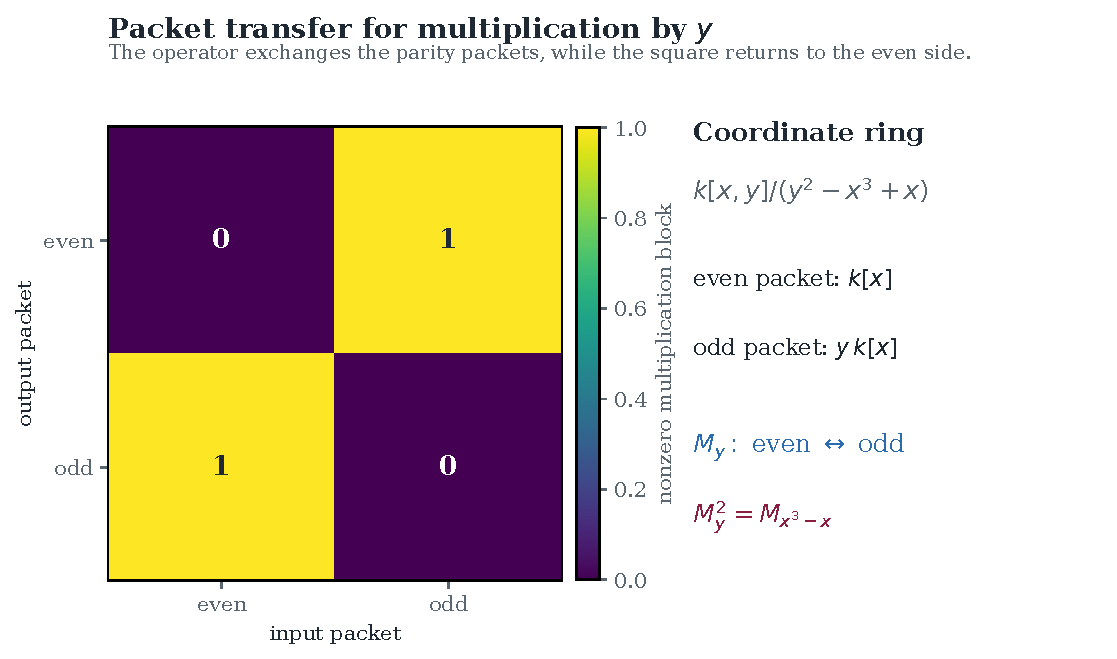
\includegraphics[width=0.61\textwidth]{08_elliptic_packet_transfer.pdf}
\caption{Multiplication by $y$ exchanges the even and odd packets. The odd-to-even transfer carries the relation weight $x^3-x$.}
\label{fig:elliptic-transfer}
\end{figure}

\subsection{Exact product law}

Write
\[
f=a_0+ya_1,
\qquad
g=b_0+yb_1.
\]
Then
\[
{
fg
=
\bigl(a_0b_0+(x^3-x)a_1b_1\bigr)
+
y\bigl(a_0b_1+a_1b_0\bigr).
}
\]
This is a two-packet convolution law. It is already visible at the linear operator level because multiplication by a fixed element is a transfer operator.

\begin{example}[Worked reduction]
Take
\[
f=x^2+y,
\qquad
g=x-y.
\]
Then
\[
\begin{aligned}
fg
&=x^3-x^2y+xy-y^2\\
&=x^3-x^2y+xy-(x^3-x)\\
&=x+(x-x^2)y.
\end{aligned}
\]
Thus
\[
P_0(fg)=x,
\qquad
P_1(fg)=(x-x^2)y.
\]
The symbolic certificate in the companion code performs the same quotient reduction exactly.
\end{example}

\subsection{What this example establishes}

The coordinate ring illustrates four distinct parts of the calculus:
\begin{enumerate}[label=(\roman*)]
\item the unit is a module seed;
\item $M_x$ and $M_y$ are address operators;
\item the curve equation is an operator relation;
\item parity in $y$ gives exact packet analysis, transfer, and reconstruction.
\end{enumerate}
It does not imply that every algebra has a one-generator algebra presentation. It shows instead that unital algebras are cyclic as modules over their full multiplication algebra.

\section{Worked signal model: a bilateral shift}

Let $\mathbb{F}\in\{\R,\C\}$ and let
\[
X=\ell^2(\Z;\mathbb F)
\]
with the explicit integer-indexed family of bounded reindexing operators
\[
(S_mx)[n]=x[n-m]
\qquad(m,n\in\Z).
\]
Thus $S_0=I$, $S_{m+r}=S_mS_r$, and $S_1$ is the usual bilateral shift. We use the standard Hilbert-space and bounded-operator conventions of \cite{conway1990}.
The impulse $\delta_0$ satisfies
\[
S_m\delta_0=\delta_m
\]
for every $m\in\Z$. Therefore finite-support sequences lie in its algebraic orbit hull and are dense in $\ell^2(\Z)$.

\begin{proposition}[Shift seed]
\label{prop:shift-seed}
For $n\in\N$, let $G(n)$ mean that some $n$-element finite seed set has dense hull under the declared family $\{S_m:m\in\Z\}$. Then
\[
{
1=\min\{n\in\N:G(n)\}.
}
\]
Equivalently, one seed suffices and no empty seed family generates densely.
\end{proposition}

\begin{proof}
The orbit of $\delta_0$ contains every standard basis vector. Their finite linear span is dense, so $G(1)$ holds. The hull of the empty seed set is zero, while $\ell^2(\Z;\mathbb F)$ is nonzero, so $G(0)$ fails. Therefore $1$ is the least admissible finite cardinality.
\end{proof}

For $N\ge1$, define residue projectors
\[
(P_{N,j}x)[n]
=
\begin{cases}
x[n],&n\equiv j\pmod N,\\0,&\text{otherwise.}\end{cases}
\]
They form an orthogonal packet system and satisfy
\[
S_1P_{N,j}=P_{N,j+1}S_1,
\]
with indices modulo $N$. The shift is therefore a cyclic transfer between residue packets.

\begin{figure}[htbp]
\centering
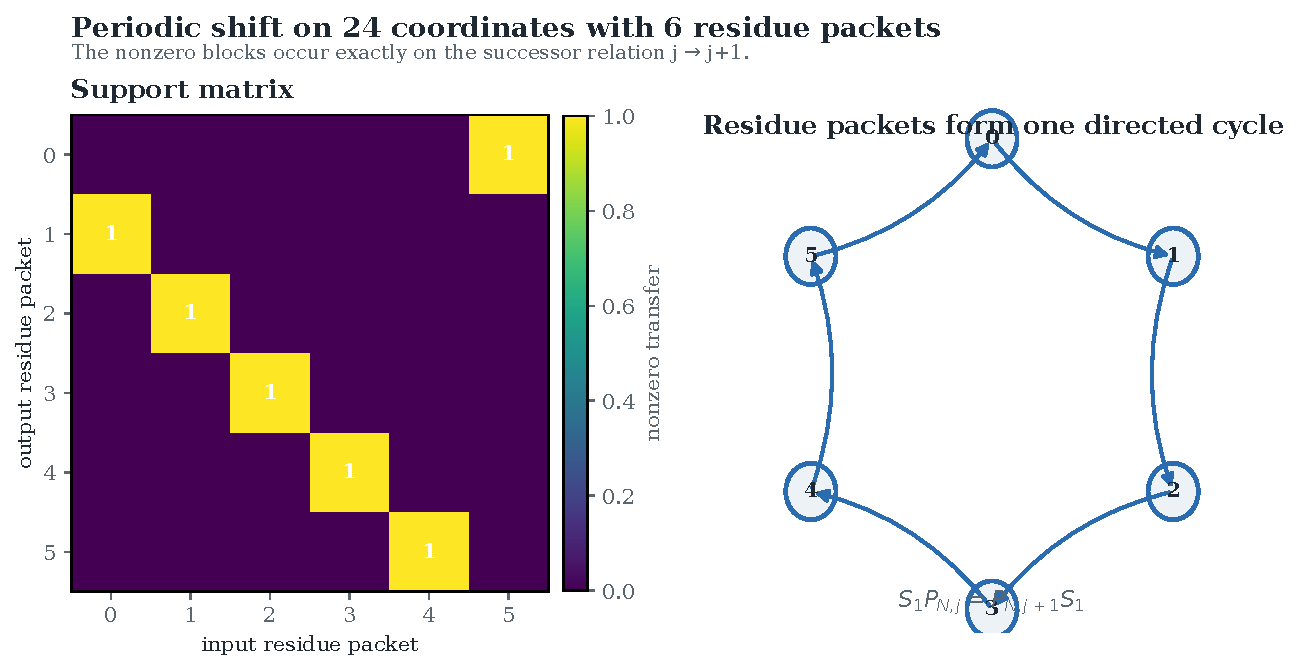
\includegraphics[width=0.66\textwidth]{07_shift_packet_transfer.pdf}
\caption{Residue-packet support in the 24-coordinate periodic shift model with six packets. Each input residue transfers into the next output residue. The infinite bilateral-shift theorem is established separately in the text.}
\label{fig:shift-transfer}
\end{figure}

\begin{boundary}
This section uses residue packets only to demonstrate the foundational transfer algebra. Nested refinement and filter-bank structures require additional definitions and are outside Paper I.
\end{boundary}

\section{Worked matrix models}

\subsection{The full matrix algebra}

Let $X=\bbk^n$ and let $\cA=M_n(\bbk)=\End_{\bbk}(X)$, with the full matrix algebra declared before a seed or target is chosen. By \cref{cor:full-matrix}, every nonzero seed is cyclic. This is the maximal linear grammar on $X$, not a compression result; under a smaller declared operator algebra, the same vector need not be cyclic.

\subsection{Companion and repeated-block operators}

For one operator $T$, \cref{thm:single-operator} turns verified primary data
into an exact minimum-seed certificate.  The numerical companion compares:
\begin{enumerate}[label=(\alph*)]
\item a nilpotent companion operator with one Jordan chain, for which the Krylov rank is $1,2,\ldots,n$;
\item two equal Jordan blocks, for which one diagonal seed produces a chain only as long as one block and then stalls.
\end{enumerate}

The observed stall is not numerical failure.  The associated
two-dimensional scalar quotient is the lower-bound certificate in
\cref{thm:single-operator}; the identification of that quotient with the
geometric-multiplicity space is the classical Jordan input stated above.

\section{Worked graph model: adjacency algebras}

Let $G$ be a nonempty finite graph with adjacency matrix $A_G$, and regard
$\bbk^{V(G)}$ as a module over $\bbk[A_G]$.  The kernel-checked general result
starts from an exact spectral certificate rather than deriving one from graph
symmetry.

\begin{corollary}[Certified graph seed number]
\label{cor:graph-rank}
Let $\bbk$ be a field and let $\Lambda$ be a nonempty finite set.  Suppose
there are pairwise distinct scalars $a_{\lambda}\in\bbk$, multiplicities
$m_{\lambda}\in\N$, and an eigenbasis
\[
\{b_{\lambda,j}:\lambda\in\Lambda,\ 1\le j\le m_{\lambda}\}
\]
of $\bbk^{V(G)}$ satisfying
\[
A_Gb_{\lambda,j}=a_{\lambda}b_{\lambda,j}.
\]
If $m_{\lambda}\le R$ for all $\lambda$ and
$m_{\lambda_*}=R$ for some $\lambda_*$, then $R$ is the least natural number
of adjacency seeds:
\[
{
R=\min\left\{r\in\N:
\begin{array}{l}
\text{there exist }s_1,\ldots,s_r\text{ with}\\[2pt]
\bbk^{V(G)}=\Span_{\bbk}
  \{p(A_G)s_j:p\in\bbk[t],\ 1\le j\le r\}
\end{array}
\right\}.
}
\]
\end{corollary}

\begin{proof}
The distinct eigenvalue labels give Lagrange polynomials that project onto
the individual eigenspace packets.  Padding one basis vector from every
packet into each of $R$ seeds gives the upper bound.  Projection to the
$m_{\lambda}$ eigenspace coordinates is a surjective scalar quotient, so any
generating family has at least $m_{\lambda}$ members for every $\lambda$.
The label $\lambda_*$ gives the matching lower bound $R$.
\end{proof}

\begin{boundary}[Spectral-classification input]
For a finite undirected graph over $\C$, the real-symmetric spectral theorem
classically supplies a certificate of the displayed kind, and the numbers
$m_{\lambda}$ are the usual eigenvalue multiplicities; see
\cite{brouwerHaemers2012}.  The formal declaration verifies the
seed-number formula from the supplied eigenbasis and distinct eigenvalue
labels.  It does not derive diagonalizability from symmetry or implement an
eigensolver.
\end{boundary}

\subsection{Path graphs}

For every field $\bbk$ and every $n\ge1$, an endpoint of $P_n$ is a cyclic
vector for the adjacency operator.  Consequently one is the least finite
adjacency-seed number:
\[
{
1=\min\left\{r\in\N:
\exists s_1,\ldots,s_r,\quad
\bbk^n=\Span_{\bbk}\{p(A_{P_n})s_j:p\in\bbk[t],\ 1\le j\le r\}
\right\}.
}
\]
Over $\C$, the familiar spectral description has the distinct eigenvalues
\[
\lambda_k=2\cos\frac{k\pi}{n+1},
\qquad 1\le k\le n,
\]
and the normalized eigenvectors have endpoint coordinate proportional to
\[
\sin\frac{k\pi}{n+1}\ne0.
\]
The all-field, kernel-checked certificate is instead combinatorial.  Let
\[
K_n=[e_1,Ae_1,\ldots,A^{n-1}e_1].
\]
Its $(i,j)$ entry counts walks of length $j-1$ from the first vertex to vertex $i$. This entry is zero when $i>j$, while the diagonal entry is one because there is a unique shortest walk of length $i-1$ from vertex $1$ to vertex $i$. Hence $K_n$ is upper triangular with unit diagonal, so
\[
\det K_n=1
\qquad(n\ge1).
\]
Thus the endpoint is cyclic for every path size, not merely for the tested range.

\begin{figure}[htbp]
\centering
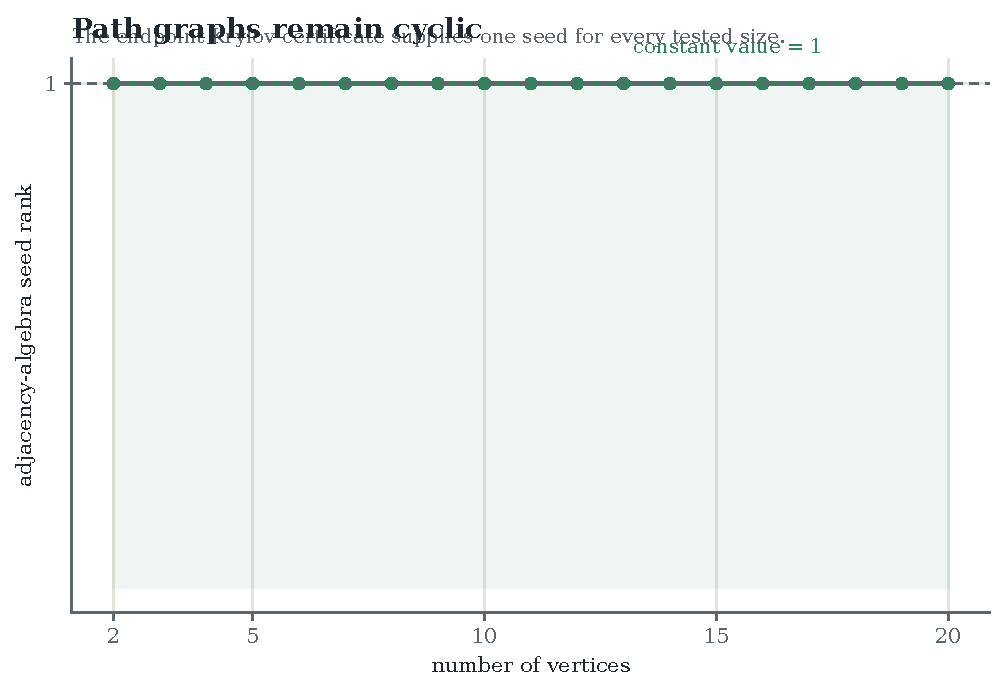
\includegraphics[width=0.75\textwidth]{05_path_graph_seed_rank.pdf}
\caption{The endpoint Krylov certificate gives every nonempty path one adjacency seed.}
\label{fig:path-rank}
\end{figure}

\subsection{Cycle graphs}

Two adjacent vertex vectors generate the adjacency module of every simple
cycle.  Over $\C$, a primitive-root Fourier quotient supplies a matching
two-dimensional scalar obstruction.  Hence, for every $n\ge3$, two is the
least finite adjacency-seed number:
\[
{
2=\min\left\{r\in\N:
\exists s_1,\ldots,s_r,\quad
\C^n=\Span_{\C}\{p(A_{C_n})s_j:p\in\C[t],\ 1\le j\le r\}
\right\}.
}
\]
To see the upper bound directly, index the vertices modulo $n$.
The identity $Ae_j=e_{j-1}+e_{j+1}$ recovers successive vertex vectors
from $e_0$ and $e_1$, over any field. For the lower bound over $\C$, let
$\zeta$ be a primitive $n$th root of unity and define
\[
q(x)=\left(\sum_{j=0}^{n-1}\zeta^j x_j,
             \sum_{j=0}^{n-1}\zeta^{-j}x_j\right).
\]
Then $q(Ax)=(\zeta+\zeta^{-1})q(x)$. The images of $e_0$ and $e_1$
are $(1,1)$ and $(\zeta,\zeta^{-1})$, which are independent because
$\zeta\ne\zeta^{-1}$ for $n\ge3$. Thus $q$ is a two-dimensional
scalar quotient, and \cref{prop:scalar-quotient-obstruction} gives the
matching lower bound.

The usual spectral description writes the eigenvalues as
\[
\lambda_k=2\cos\frac{2\pi k}{n},
\qquad 0\le k<n.
\]
The values for $k$ and $n-k$ coincide. Apart from the simple characters at $k=0$ and, for even $n$, $k=n/2$, the eigenspaces occur in pairs. Therefore the maximum eigenspace multiplicity is two, although some eigenspaces have multiplicity one, and
the certified minimum above is two.

\begin{figure}[htbp]
\centering
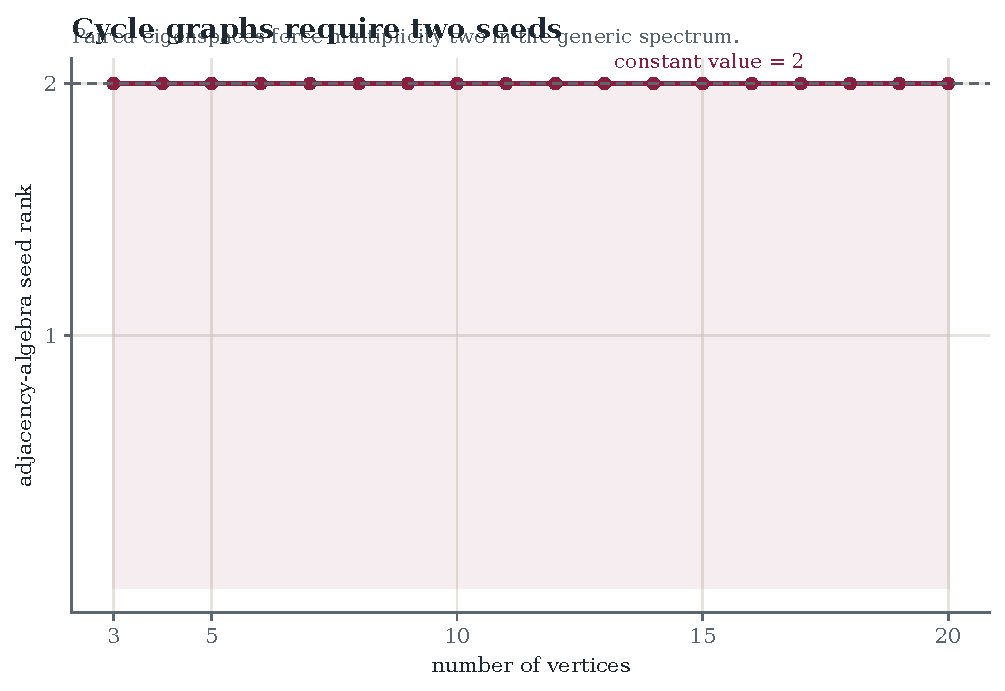
\includegraphics[width=0.75\textwidth]{06_cycle_graph_seed_rank.pdf}
\caption{Cycle graphs have maximum adjacency-eigenspace multiplicity two and therefore require two adjacency seeds, although one or two exceptional eigenspaces are simple.}
\label{fig:cycle-rank}
\end{figure}

The path and cycle examples use nearly identical local operators.  Their
kernel-checked minimum finite seed numbers differ because the path has an
endpoint Krylov basis, whereas the cycle has a two-dimensional Fourier
quotient obstruction.

\section{The common operator language}

The preceding examples can be written without changing the foundational notation.

\begin{longtable}{L{0.12\textwidth}L{0.13\textwidth}L{0.19\textwidth}L{0.17\textwidth}L{0.16\textwidth}}
\caption{Foundational realizations of the common operator language.}\label{tab:dictionary}\\
\toprule
Realization & Seed & Operator grammar & Packets & Completion or quotient \\
\midrule
\endfirsthead
\toprule
Realization & Seed & Operator grammar & Packets & Completion or quotient \\
\midrule
\endhead
Coordinate ring & $1$ & $M_x,M_y$ & even/odd $y$ degree & quotient by $y^2-x^3+x$ \\
Shift system & $\delta_0$ & $(S_m)_{m\in\Z}$ & residue classes of $n$ & $\ell^2$ closure \\
Full matrix module & $s\ne0$ & $M_n(\bbk)$ & chosen idempotents & finite-dimensional \\
Single operator & $s_1,\ldots,s_r$ & $\bbk[T]$ & primary or spectral & finite-dimensional \\
Graph adjacency & vertex seeds & $\bbk[A_G]$ & eigenspaces & finite-dimensional \\
Typed grammar & vertex seeds & path algebra $\bbk Q/I$ & vertex idempotents & relation quotient \\
\bottomrule
\end{longtable}

The invariant content is:
\[
{
\begin{aligned}
&\text{generated hull: }\Hull_{\cA}(S),\\
&\text{seed complexity: }\srank_{\cA}(X),\\
&\text{packet coordinates: }x\leftrightarrow(P_{\alpha}x)_{\alpha},\\
&\text{operator coordinates: }T\leftrightarrow(P_{\beta}TP_{\alpha})_{\beta,\alpha},\\
&\text{relations: }F^m/N_S,\\
&\text{coordinate invariance: }P_{\alpha}\mapsto UP_{\alpha}U^{-1},\\
&\text{realization: }\Phi A=\varphi(A)\Phi.
\end{aligned}
}
\]

\begin{figure}[htbp]
\centering
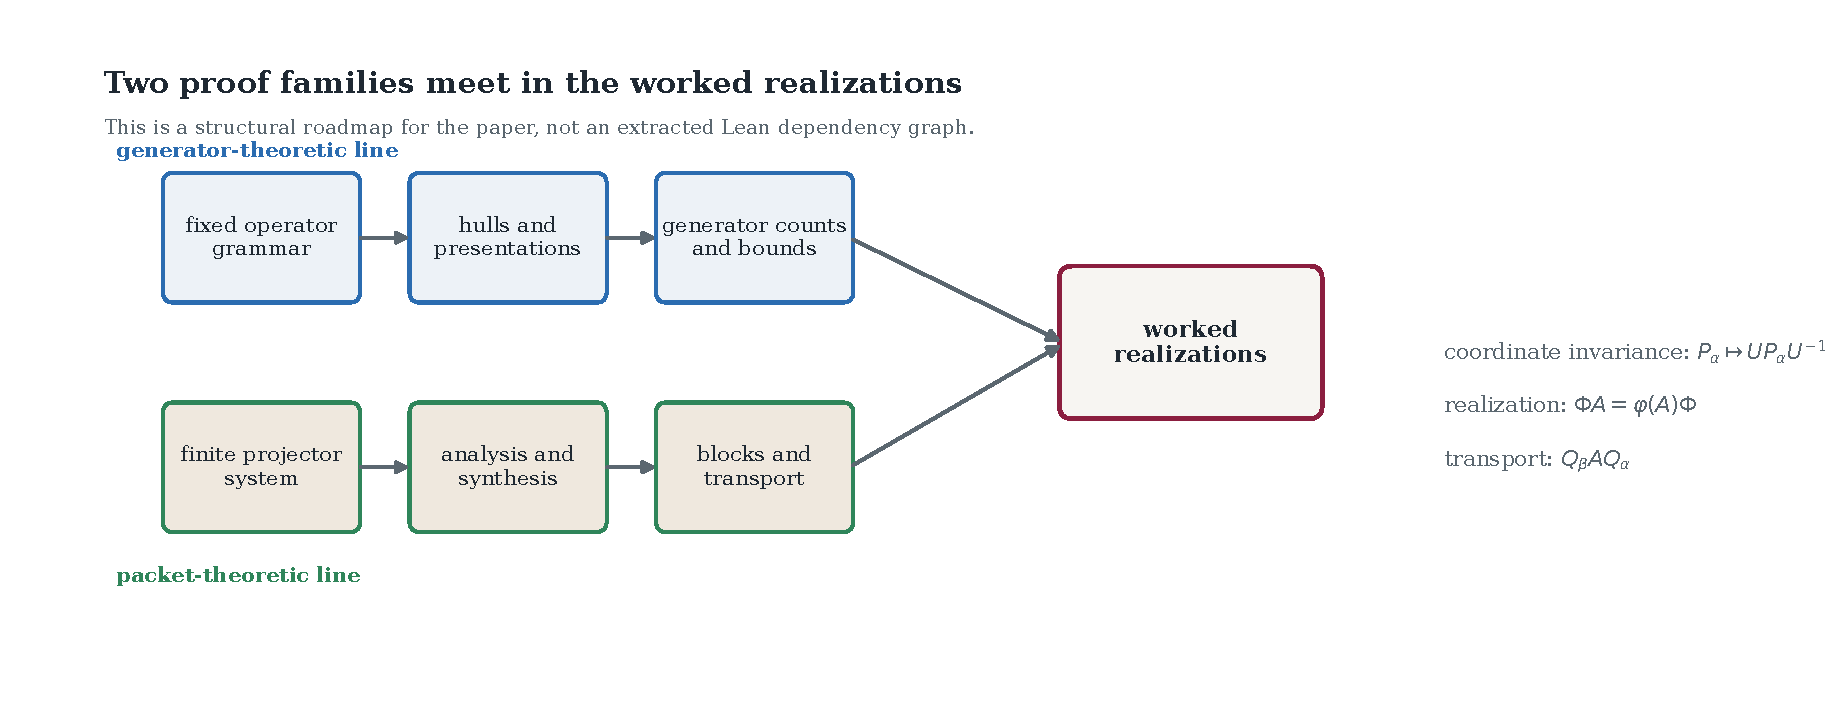
\includegraphics[width=0.96\textwidth]{10_theorem_dependency.pdf}
\caption{Structural overview of the two proof families. The generator and packet arguments meet in the worked realizations. This diagram is not an exhaustive graph of Lean declaration dependencies.}
\label{fig:dependency}
\end{figure}

\section{Computational certificates}

The accompanying Python package is not used as a substitute for proof. It provides exact symbolic checks and finite numerical regression tests for formulas already proved. The computed ranges and random seeds are recorded explicitly. These checks do not extend a theorem beyond its hypotheses or certify an unrestricted numerical implementation. The journal companion also tests integer counts beyond floating-point precision and rejects the unsupported complex-symmetric spectral shortcut.

\subsection{Test suite}

The test suite checks:
\begin{enumerate}[label=(\roman*)]
\item projector idempotence, annihilation, and completeness;
\item exact vector analysis and synthesis;
\item exact operator reconstruction from all transfer blocks;
\item coordinate transport under a dense random similarity transform;
\item cyclicity of a companion operator;
\item the two-seed obstruction for repeated Jordan blocks;
\item the semisimple multiplicity formula in representative cases;
\item full orbit dimension for two representative nonzero seeds under the full matrix algebra;
\item exact reduction and packet multiplication in the elliptic coordinate ring;
\item seed ranks of path and cycle adjacency modules over the reported finite ranges;
\item the cyclic residue transfer pattern of a finite shift.
\end{enumerate}

\subsection{Recorded results}

\begin{table}[htbp]
\centering
\caption{Representative computed checks from the journal-edition run.}
\label{tab:results}
\begin{tabular}{L{0.57\textwidth}r}
\toprule
Quantity & Result \\
\midrule
Projector idempotence residual & $0$ \\
Projector annihilation residual & $0$ \\
Projector completeness residual & $0$ \\
Operator reconstruction residual & $0$ \\
Transported-projector residual, maximum & $1.85\times10^{-15}$ \\
Companion seed rank & $1$ \\
Two equal Jordan blocks, seed rank & $2$ \\
$M_3(\C)$ acting on seven copies, seed rank & $3$ \\
Sampled path graph seed ranks, $2\le n\le12$ & $1$ \\
Sampled cycle graph seed ranks, $3\le n\le12$ & $2$ \\
Full $M_4(\R)$ orbit dimensions for two sampled nonzero seeds & $4,4$ \\
Automated tests & $33/33$ passed \\
\bottomrule
\end{tabular}
\end{table}

The finite shift pattern recovered by the experiment is
\[
\begin{pmatrix}
0&0&0&1\\
1&0&0&0\\
0&1&0&0\\
0&0&1&0
\end{pmatrix},
\]
which is the exact packet adjacency of a cyclic four-phase transfer.

\subsection{Algorithms}

The Lean component proves mathematical specifications for the following
finite constructions.  These statements establish termination and
correctness at the level of subspaces, block tables, and exact certificates;
they do not assert code extraction or a particular backend's performance.

\begin{construction}[Orbit-hull closure specification]
\label{con:orbit-hull-algorithm}
Let $V$ be finite-dimensional, let $(O_i)_{i\in I}$ be a finite operator
family, and let $S\subseteq V$.  Define
\[
W_0=\Span_{\bbk}S,
\qquad
W_{n+1}=W_n+\sum_{i\in I}O_i(W_n).
\]
Then there is an $n\in\N$ such that
\[
W_{n+1}=W_n
\qquad\text{and}\qquad
W_n=\Hull_{(O_i)}(S),
\]
where the right side is the least subspace containing $S$ and invariant under
every $O_i$.  Thus the ascending subspace iteration terminates and its stable
value is exactly the finite operator hull.
\end{construction}

\begin{construction}[Transfer-block table specification]
\label{con:transfer-block-algorithm}
Given finite projector systems $(P_i)_{i\in I}$ and $(Q_j)_{j\in J}$ and a
linear map $T$, form the table
\[
B_{ji}=Q_jTP_i.
\]
Its assembly reconstructs the input map exactly,
\[
\sum_{j\in J}\sum_{i\in I}B_{ji}=T,
\]
and its reported support relation is exactly
$\{(i,j):B_{ji}\ne0\}$.  The latter equality is the specification of the
transfer-graph output, not a claim that Lean extracts a decidable edge-list
routine for every coefficient field.
\end{construction}

\begin{construction}[Certified exact graph seed-rank specification]
\label{con:exact-graph-seed-rank}
For a finite square matrix $A$ over a field $K$, define the noncomputable exact
spectral quantity
\[
r_{\mathrm{spec}}(A)
=
\max_{\mu\in\Spec_K(A)}
\dim_K\ker(A-\mu I),
\]
with value zero for an empty spectrum.  Suppose an exact certificate supplies
a finite eigenbasis indexed by labels and multiplicities, the eigenvalue
equations, a multiplicity bound attained by one label, projector polynomials
that extract the padded eigenbasis generators, coverage of every spectral
value by a label, equality of the declared and actual eigenspace dimensions,
and membership of the maximizing eigenvalue in the spectrum.  Then
$r_{\mathrm{spec}}(A)$ is the least natural number of polynomial-orbit seeds
for $A$.

This is a verified certificate checker/specification.  It does not construct
the eigenbasis, prove that a symmetric matrix is diagonalizable, or implement
an exact eigensolver.  The companion Python code performs symbolic
computations in the reported finite graph range; the all-size path and cycle
results are proved separately above.
\end{construction}

\section{Formal verification record}

The accompanying formal development uses Lean 4.34.0-rc2 \cite{demouraUllrich2021}
and a pinned Mathlib revision \cite{mathlib2020}. Its 35-row contract links 32 registered mathematical
claims and three mathematical algorithm specifications to 84 named targets.
Some targets are construction definitions rather than theorem declarations;
the target count is not a count of 84 independent theorems. The map records
the hypotheses and exclusions of each result in
\path{formalization/lean/LEAN_THEOREM_MAP_v1.0.2.md}.

For this journal edition, the project sources were rebuilt in a fresh object
directory using a focused import module. The eight former blanket Mathlib
imports were replaced, but no existing formal statement or proof body was
changed. This reduces the memory required to check the development. The
pinned Mathlib dependency cache was reused, not independently rebuilt.

\begingroup
\small
\setlength{\tabcolsep}{3pt}
\begin{longtable}{L{0.24\textwidth}L{0.29\textwidth}L{0.36\textwidth}}
\caption{Principal modules in the accompanying Lean development.}
\label{tab:lean-modules}\\
\toprule
Module & Representative declaration & Checked scope \\
\midrule
\endfirsthead
\toprule
Module & Representative declaration & Checked scope \\
\midrule
\endhead
\texttt{SeedRankBasics}; \texttt{SeedRankOperations}
& \path{cyclic_iff_seedRank_eq_one}; \path{seedRank_tensorProduct_le_mul}
& Cardinal seed rank, free presentations, cyclicity, semilinear functoriality, image-algebra invariance, direct sums, tensor products, and scalar quotients. \\
\texttt{SemisimpleSeedRank}; \texttt{SemisimpleCompletion}
& \path{semisimple_seedRank_eq_maxCeilDiv_of_equivalences}
& One-block and finite-product generator formulas, transport through chosen split algebra and compatible module equivalences, full matrices, and multiplicity obstruction. \\
\texttt{SingleOperatorGraph}
& \path{singleOperator_seedNumber_isLeast_of_primary_decomposition}
& Certified primary and diagonalizable least-seed formulas, cyclicity wrappers, every nonempty path, and every complex cycle of size at least three. \\
\texttt{ExactCoordinates}; \texttt{PaperIBlockCompletion}
& \texttt{exactPacketCoordinates}; \path{transferBlock_comp_linearMap}
& Exact packet coordinates, operator reconstruction, block composition, and support identities. \\
\texttt{PacketNaturality}\allowbreak\texttt{Completion}
& \path{strict_naturality_package}
& Packetwise equality, all finite powers, full dependent block algebra, dimension, reachability, conjugation, strict naturality, and the typed quiver certificate. \\
\texttt{TopologicalCompletion}
& \path{topological_packet_isomorphism}; \path{concreteBilateralShift_seedCardinality_isLeast}
& Closed packet ranges, standard product-norm equivalence, completion, adjoints, closure obstruction, dense transport, packet descent, and the concrete bilateral shift. \\
\texttt{EllipticAlgorithms}
& \path{My_sq_eq_Mx_cube_sub_Mx}; \path{orbitHull_algorithm_terminates_and_correct}
& Quotient normal form, coordinate projectors and product law, the unit seed, operator relation, orbit iteration, transfer table, and certified spectral-rank specification. \\
\texttt{KernelAudit}
& 84 mapped \texttt{\#print axioms} commands; fail-closed namespace command
& Concrete smoke tests, complete mapped-declaration reports, and a namespace-wide trust gate. \\
\bottomrule
\end{longtable}
\endgroup

The fresh checks compile all 20 local modules, resolve all 84 mapped
targets, and run the fail-closed audit over 1,126 project declarations,
including definitions and generated helpers. The reported transitive axiom
dependencies are confined to \texttt{propext}, \texttt{Classical.choice},
and \texttt{Quot.sound}. Separate negative controls require Lean to reject
a false natural-number equality and to reject a theorem placeholder when
warnings are treated as errors. Commands, source hashes, type signatures,
and unedited compiler output are included in the verification supplement.

The earlier v1.2.1 record reported an 8,883-job aggregate build. That is
historical evidence, not the job count of this audit. The present checks
establish acceptance of the accompanying local declarations relative to the
pinned imported library. They do not certify every sentence of exposition,
independent mathematical novelty, or a general executable eigensolver.

The certificate boundary is material. Lean checks the implications from chosen split decompositions, primary data, eigenbases, projector polynomials, quotient maps, and spectrum-coverage certificates. It does not construct those certificates from Wedderburn--Artin, Jordan, the spectral theorem, graph symmetry, or an eigensolver. Likewise, the Lean elliptic-coordinate module checks the quotient algebra and operator identities, not projective smoothness or genus.

\section{Classical inputs, new organization, and claim boundary}

\subsection{Classical mathematical inputs}

The following are established ingredients:
\begin{itemize}
\item modules over associative algebras and path algebras;
\item cyclic modules and companion matrices;
\item Jordan decomposition and primary decomposition;
\item Wedderburn's structure theorem for finite-dimensional semisimple algebras;
\item direct-sum and tensor-product constructions;
\item idempotent decompositions and block matrices;
\item spectral theory of symmetric graph adjacency matrices.
\end{itemize}

These facts are not renamed as new theorems. In the kernel-checked statements, their outputs appear as explicit inputs: a chosen split algebra equivalence, a compatible module equivalence, primary block generators, extraction polynomials, scalar quotient maps, an eigenbasis, or exact spectrum-coverage data. Lean verifies the conclusions from those certificates. It does not, in this release, derive the certificates from the classification theorems themselves. This distinction is part of the formal claim boundary rather than a hidden implementation detail.

\subsection{Claim-status ledger}

In \cref{tab:claim-status}, \texttt{P} means that a proof is supplied in this paper, without implying historical novelty; \texttt{C} means classical or reformulated from established theory; \texttt{I} means that the companion package checks finite computed instances; and \texttt{L} means that the stated scope has been checked in the accompanying Lean component. Each of the 35 registered rows carries \texttt{L} at its specified scope. A Lean entry applies only to the scope named in the final column; exact declaration names appear in \path{formalization/lean/LEAN_THEOREM_MAP_v1.0.2.md}.

The full ledger appears in Appendix~\ref{app:claim-ledger}. Its row
identifiers are unchanged from the v1.2.1 contract, so the journal article
and the archived formal record can be compared without renumbering results.

\subsection{Framework-level contribution}

The organizing choice is to keep the acting algebra, generated module,
relations, projector coordinates, and realization maps explicit throughout.
The same seed-rank and transfer identities can then be used in each worked
model without changing their meaning. The definitions and formulas retain
their classical module-theoretic content; the common presentation and
source-linked proofs make their hypotheses easier to compare and reuse.

This is a framework and formalization contribution. It is not a priority
claim for minimal generator numbers, idempotent decompositions, or cyclic
module theory. A broader comparison with systems theory, quiver
representations, and multiresolution methods requires separate treatment.

\subsection{Roadmap boundary}

Nested refinement, nonlinear packet maps, and domain-specific realizations are roadmap items. They are not used to justify any theorem in Paper I, and no Paper I result depends on a conjecture.

\section{Conclusion}

A fixed operator algebra turns a generation claim into a question about a
module. A finite projector family gives exact coordinates on that module,
and the transfer blocks recover both the operator and its composition law.
Relations determine the presentation; topology determines which closures
or completions are justified.

The multiplicity formulas show why these distinctions matter. A cyclic
component may require several generators when it is repeated under a shared
action. A path has an endpoint Krylov basis, whereas a complex cycle has a
two-dimensional scalar quotient that prevents one-seed generation. The
number of seeds is therefore a property of the action, not of a preferred
coordinate description.

The results collected here provide a common starting point for subsequent
realizations: a specified grammar, a generated module, a minimum generator
count, packet coordinates, and exact transport identities. The formal record
preserves the assumptions on which those statements depend. Extensions can
build on this core without confusing a chosen decomposition with a proof
that such a decomposition exists.

\appendix

\section{Notation and status conventions}

\begin{longtable}{L{0.21\textwidth}L{0.70\textwidth}}
\caption{Notation used throughout Paper I.}\label{tab:notation}\\
\toprule
Symbol & Meaning \\
\midrule
\endfirsthead
\toprule
Symbol & Meaning \\
\midrule
\endhead
$Q$ & quiver of operator types and primitive typed operations \\
$\bbk Q/I$ & path algebra with declared relations \\
$X$ & ambient module or topological vector space \\
$S$ & seed family \\
$\cA$ & unital operator algebra acting on $X$ \\
$\Hull_{\cA}(S)$ & algebraic operator hull \\
$\srank_{\cA}(X)$ & minimal number of module seeds \\
$P_{\alpha}$ & packet projector \\
$X_{\alpha}=P_{\alpha}X$ & packet space \\
$T_{\beta\alpha}=P_{\beta}TP_{\alpha}$ & transfer block \\
$\mathcal A_{\cP}$ & packet analysis map \\
$\mathcal S_{\cP}$ & packet synthesis map \\
$\Phi A=\varphi(A)\Phi$ & intertwining condition \\
\bottomrule
\end{longtable}

Environment labels describe a statement's local role; the independent proof and machine-evidence classifications are the \texttt{P/C/I/L} codes in \cref{tab:claim-status}. A \emph{boundary} records something intentionally not claimed. Roadmap items are not theorems, and no theorem in Paper I is marked conjectural.

\section{Proof dependency map}

The logical order is:
\[
\begin{aligned}
&\text{typed grammar and path algebra}\\
&\qquad\Downarrow\\
&\text{generated hull and free presentation}\\
&\qquad\Downarrow\\
&\text{seed rank and functorial bounds}\\
&\qquad\Downarrow\\
&\text{semisimple and single-operator formulas},
\end{aligned}
\]
while independently
\[
\begin{aligned}
&\text{idempotent packet system}\\
&\qquad\Downarrow\\
&\text{analysis/synthesis and transfer blocks}\\
&\qquad\Downarrow\\
&\text{coordinate transport and naturality}.
\end{aligned}
\]
The two branches meet in the worked models, where the generated module is explicitly resolved into packet coordinates.

\section{Reproducibility layout}

The journal source package is organized as follows:
\begin{lstlisting}
Komorebi_Paper_I_Journal_v1.3.0/
  README.md
  SHA256SUMS.txt
  paper/                 LaTeX source, PDF, figures
  formalization/lean/    pinned Lean sources and claim map
  code/python/           symbolic and numerical companion
  results/               regenerated examples and figure record
  verification/          compiler logs, types, tests, environment
  review/                corrections and source comparisons
  provenance/            original release record
  scripts/               repeatable verification and build tools
\end{lstlisting}

The verification supplement records the exact source hashes and observed
outcomes of each executed check. The Python figure-and-example command
records only the outputs it produces; it does not report that Lean, tests,
or PDF review have passed merely because those checks passed in a previous
release. Test results, compiler acceptance, and visual inspection have
separate records.

The formal development is pinned by \texttt{lean-toolchain} and
\texttt{lake-manifest.json}. The fresh audit reuses matching dependency
objects and rebuilds the local sources. Reproducing the full dependency
build is a distinct operation. The manuscript's written proofs, the
source-to-statement correspondence, and the compiler checks likewise
remain separate parts of the review.

\section{Claim-status ledger}\label{app:claim-ledger}

\begingroup
\small
\setlength{\tabcolsep}{3pt}
\begin{longtable}{L{0.16\textwidth}L{0.25\textwidth}L{0.10\textwidth}L{0.38\textwidth}}
\caption{Status and verification scope of the principal claims in Paper I.}
\label{tab:claim-status}\\
\toprule
Section & Claim & Status & Verification scope \\
\midrule
\endfirsthead
\toprule
Section & Claim & Status & Verification scope \\
\midrule
\endhead
Free presentations & Universal one-seed presentation & \texttt{C/P/L} & Exact algebraic quotient and generation criterion; dense-isometric completion and bounded intertwining are also checked. \\
Free presentations & Multi-seed presentation & \texttt{C/P/L} & Exact free-module quotient plus the least finite free-rank characterization for finite modules. \\
Seed rank & Cyclic characterization & \texttt{C/P/L} & Exact unrestricted nonzero cardinal-valued equivalence, with the zero-module convention separate. \\
Seed rank & Quotient monotonicity & \texttt{C/P/L} & Exact for a surjective semilinear map along an arbitrary scalar homomorphism. \\
Seed rank & Isomorphism invariance over the image algebra & \texttt{C/P/L} & Exact for the literal image algebra; full target equality requires scalar-map surjectivity. \\
Seed rank & Shared direct-sum bound & \texttt{C/P/L} & Exact cardinal bound for the diagonal action of one algebra. \\
Seed rank & Independent direct-sum formula & \texttt{C/P/L} & Exact cardinal equality for the coordinatewise product-algebra action. \\
Seed rank & Tensor-product bound & \texttt{C/P/L} & Exact over a common commutative base with the stated scalar-tower action. \\
Seed rank & Scalar quotient obstruction & \texttt{C/P/L} & Exact for a character and a surjective semilinear map to a finite scalar module. \\
Semisimple modules & Semisimple multiplicity formula & \texttt{C/P/L} & Exact from chosen split algebra and compatible semilinear module equivalences; classification existence is external. \\
Semisimple modules & Full matrix algebra & \texttt{C/P/L} & Exact seed rank one and constructive cyclicity of every nonzero vector. \\
Semisimple modules & Multiplicity obstruction & \texttt{C/P/L} & Exact cardinal formula $\lceil m/d\rceil$ for the diagonal full-matrix action. \\
One operator & Certified single-operator seed number & \texttt{C/P/L} & Exact least polynomial-orbit count and canonical $\bbk[T]$ seed rank from explicit primary certificates. \\
One operator & Certified cyclic matrix criterion & \texttt{C/P/L} & Stronger four-condition chain once the geometric/block and minpoly/charpoly bridges are supplied: the checked implication does not need the separately inherited finite-label hypothesis. \\
Packet coordinates & Exact packet coordinates & \texttt{C/P/L} & Exact two-sided analysis--synthesis equivalence for finite projector families. \\
Packet coordinates & Packetwise equality & \texttt{C/P/L} & Exact iff: equality is detected by all packet projectors. \\
Topological packets & Topological packet isomorphism & \texttt{C/P/L} & Exact closed ranges and continuous linear equivalence for the standard finite product norm. \\
Topological packets & Completion preserves a finite packet split & \texttt{C/P/L} & Exact: $\closure{P_iM}=P_iX$ for any bounded idempotent, with no invariance of $M$ required. \\
Transfer blocks & Exact operator reconstruction & \texttt{C/P/L} & Exact operator identity. \\
Transfer blocks & Packet matrix multiplication & \texttt{C/P/L} & Exact composition identity. \\
Transfer blocks & Packet powers & \texttt{C/P/L} & Exact finite path expansion for every natural power, including the zeroth power. \\
Transfer blocks & Adjoint reversal & \texttt{C/P/L} & Stronger: bounded self-adjoint packet maps suffice; orthogonal-projector structure is not otherwise used. \\
Transfer blocks & Algebraic full block representation & \texttt{C/P/L} & Exact dependent block-algebra equivalence, arbitrary-block synthesis, and output-first multiplication law. \\
Transfer blocks & Dimension count & \texttt{C/P/L} & Exact finite-dimensional packet-sum and square formulas. \\
Transfer support & Algebraic packet support pattern & \texttt{C/P/L} & Exact reflexivity and transitivity iff statements for arbitrary nontrivial packet ranges. \\
Reachability & Reachability obstruction & \texttt{C/P/L} & Exact algebraic reachable-support theorem and bounded-projector closure corollary. \\
Coordinate transport & Coordinate transport & \texttt{C/P/L} & Exact blocks, edges, and reachability under conjugation. \\
Naturality & Naturality of generation and packets & \texttt{C/P/L} & Exact strict package; full edge/zero-pattern correspondence uses bijective structure maps. \\
Dense realizations & Dense realization theorem & \texttt{C/P/L} & Exact for normed spaces, bounded operator families, and a surjective continuous intertwiner; packet range descends separately. \\
Typed quiver & Typed reachability certificate & \texttt{P/L} & Exact displayed finite model: $BA=I$, missing kernel direction, no $U$-only generation, and two-seed generation. \\
Bilateral shift & Shift seed & \texttt{C/P/L} & Exact explicit integer-power grammar on $\ell^2(\Z)$; least finite dense-generating cardinality is one. \\
Graph model & Certified spectral seed number & \texttt{C/P/L} & Exact from a supplied distinct-label eigenbasis; path one and complex-cycle two are unconditional all-size theorems. \\
Algorithms & Orbit-hull iteration & \texttt{C/P/I/L} & Exact stabilization and least-invariant-hull specification in finite dimension; no extraction or performance claim. \\
Algorithms & Transfer-block table & \texttt{C/P/I/L} & Exact table reconstruction and definitional support specification; no edge-list implementation claim. \\
Algorithms & Certified exact graph rank & \texttt{C/P/I/L} & Exact noncomputable spectrum maximum from supplied spectral certificates; no verified eigensolver claim. \\
\bottomrule
\end{longtable}
\endgroup

\begingroup
\small
\begin{thebibliography}{99}

\bibitem{assemSimsonSkowronski2006}
I.~Assem, D.~Simson, and A.~Skowro{\'n}ski,
\emph{Elements of the Representation Theory of Associative Algebras, Volume 1: Techniques of Representation Theory},
London Mathematical Society Student Texts 65,
Cambridge University Press, Cambridge, 2006.
\href{https://doi.org/10.1017/CBO9780511614309}{doi:10.1017/CBO9780511614309}.

\bibitem{brouwerHaemers2012}
A.~E.~Brouwer and W.~H.~Haemers,
\emph{Spectra of Graphs},
Universitext, Springer, New York, 2012.
\href{https://doi.org/10.1007/978-1-4614-1939-6}{doi:10.1007/978-1-4614-1939-6}.

\bibitem{conway1990}
J.~B.~Conway,
\emph{A Course in Functional Analysis},
second edition, Graduate Texts in Mathematics 96,
Springer, New York, 1990.
\href{https://doi.org/10.1007/978-1-4757-4383-8}{doi:10.1007/978-1-4757-4383-8}.

\bibitem{hornJohnson2012}
R.~A.~Horn and C.~R.~Johnson,
\emph{Matrix Analysis},
second edition, Cambridge University Press, Cambridge, 2012.
\href{https://doi.org/10.1017/CBO9781139020411}{doi:10.1017/CBO9781139020411}.

\bibitem{lam2001noncommutative}
T.~Y.~Lam,
\emph{A First Course in Noncommutative Rings},
second edition, Graduate Texts in Mathematics 131,
Springer, New York, 2001.
\href{https://doi.org/10.1007/978-1-4419-8616-0}{doi:10.1007/978-1-4419-8616-0}.

\bibitem{lam1999modules}
T.~Y.~Lam,
\emph{Lectures on Modules and Rings},
Graduate Texts in Mathematics 189,
Springer, New York, 1999.
\href{https://doi.org/10.1007/978-1-4612-0525-8}{doi:10.1007/978-1-4612-0525-8}.

\bibitem{roman2008}
S.~Roman,
\emph{Advanced Linear Algebra},
third edition, Graduate Texts in Mathematics 135,
Springer, New York, 2008.
\href{https://doi.org/10.1007/978-0-387-72831-5}{doi:10.1007/978-0-387-72831-5}.

\bibitem{schaeferWolff1999}
H.~H.~Schaefer and M.~P.~Wolff,
\emph{Topological Vector Spaces},
second edition, Graduate Texts in Mathematics 3,
Springer, New York, 1999.
\href{https://doi.org/10.1007/978-1-4612-1468-7}{doi:10.1007/978-1-4612-1468-7}.

\bibitem{silverman2009}
J.~H.~Silverman,
\emph{The Arithmetic of Elliptic Curves},
second edition, Graduate Texts in Mathematics 106,
Springer, New York, 2009.
\href{https://doi.org/10.1007/978-0-387-09494-6}{doi:10.1007/978-0-387-09494-6}.


\bibitem{demouraUllrich2021}
L. de Moura and S. Ullrich,
\emph{The Lean 4 Theorem Prover and Programming Language},
in Automated Deduction---CADE 28, Lecture Notes in Computer Science 12699,
Springer, Cham, 2021, pp. 625--635.
\href{https://doi.org/10.1007/978-3-030-79876-5_37}{doi:10.1007/978-3-030-79876-5\_37}.

\bibitem{mathlib2020}
The mathlib Community,
\emph{The Lean Mathematical Library},
in Proceedings of the 9th ACM SIGPLAN International Conference on Certified
Programs and Proofs, ACM, 2020, pp. 367--381.
\href{https://doi.org/10.1145/3372885.3373824}{doi:10.1145/3372885.3373824}.

\end{thebibliography}
\endgroup



\end{document}
